%                                                                 aa.dem
% AA vers. 8.3, LaTeX class for Astronomy & Astrophysics
% demonstration file
%                                                       (c) EDP Sciences
%-----------------------------------------------------------------------

%\documentclass{aa}
\documentclass[referee]{aa}        % for a referee version
%\documentclass[onecolumn]{aa}      % for a paper on 1 column
%\documentclass[longauth]{aa}       % for the long lists of affiliations
%\documentclass[rnote]{aa}          % for the research notes
%\documentclass[letter]{aa}         % for the letters
%\documentclass[bibyear]{aa}        % if the references are not structured
                                    % according to the author-year
                                    % natbib style

%%%%%%%%%%%%%%%%%%%%%%%%%%%%%%%%%%%%%%%%
\usepackage{natbib}
\usepackage{graphicx}
\usepackage{txfonts}
\usepackage{hyperref}
\hypersetup{
    colorlinks=true,   %% links colored instead of frames
    urlcolor=blue,     %% external hyperlinks
    linkcolor=red,     %% internal latex links (eg Fig)
    citecolor=blue,
}
\usepackage{multirow}
\usepackage{booktabs}

%%%%%%%%%%%%%%%%%%%%%%%%%%%%%%%%%%%%%%%%
% To add links in your PDF file, use the package "hyperref"
% with options according to your LaTeX or PDFLaTeX drivers.

\begin{document}
  \title{Comparison of multi-frequency positions of extra-galactic sources}
%   \subtitle{I. Overviewing the $\kappa$-mechanism}
  \author{N. Liu\inst{1}
     \and
          S. B. Lambert\inst{2}
          %\fnmsep
          \and
          N. Jiang\inst{1}
          \and
          C.-Y. Ding\inst{1}
          \and
          Z. Zhu\inst{1}
          \and
          J.-C. Liu\inst{1}
        %   \thanks{Just to show the usage of the elements in the author field}
          }

  \institute{School of Astronomy and Space Science,
   		     Key Laboratory of Modern Astronomy and Astrophysics (Ministry of Education), Nanjing University, Nanjing, P. R. China\\
              \email{zhuzi@nju.edu.cn}
         \and
             SYRTE, Observatoire de Paris,
             Universit\'e PSL, CNRS, Sorbonne Universit\'e, LNE, Paris, France\\
             \email{sebastien.lambert@obspm.fr}
            %  \thanks{The university of heaven temporarily does not
                    %  accept e-mails}
             }

  \date{Received; accepted}


  \abstract
  % context heading (optional)
  % {} leave it empty if necessary
   {
       Previous comparisons of the \textit{Gaia} and radio positions measured by the very long baseline interferometry (VLBI) at $X$-band probe the structure of the milli-arcsecond (mas) scale of Active Galactic Nucleus.
       But the available VLBI positions at high frequencies are less tapped.
   }
  % aims heading (mandatory)
   {
       We aim to study the multi-frequency position of extra-galactic sources, complementary to previous studies.}
  % methods heading (mandatory)
   {
       We compared the absolute positions measured at four different bands,
       that is, the optical position from the {\it Gaia} Data Release 2 and three radio positions at $X$-, $K$-, and $Ka$-band from the ICRF3 catalog, for 488 common sources.
       We first aligned the $K$-band, $Ka$-band, and \textit{Gaia} catalogs onto the $X$-band frame.
       Then we studied the frequency-position relation and correlation of radio-to-optical offsets determined at different radio bands
       with the magnitude, source morphological properties, and relativistic jet properties.
   }
  % results heading (mandatory)
   {
       The deviation amongst radio-to-optical offsets determined at different radio bands is less than 0.54~mas for 95\% of the sample.
       The large radio-to-optical offset appears to favor faint quasars but is well explained by their formal uncertainty.
       We found that for 55 sources, the $K$-band, $Ka$-band, and \textit{Gaia} positions are on the same side of the $X$-band.
       However, this position-alignment relation is vulnerable to global systematics.
       For 22 sources with four-band positions aligned and also with available jet direction determination, more than half of them have a radio-to-optical vector parallel to the jet.
       %A simulation considering the position error ellipses suggests that four positions of extra-galactic objects agree at a level of 0.1~mas.
       %, even though small offsets could be obtained from the given positions in catalogs
   }
  % conclusions heading (optional), leave it empty if necessary
   {
       The source structure might not perturb the radio-to-optical offset measured at $X$-band much.
       The selection of sources for the link between the ICRF and \textit{Gaia}-CRF is not necessarily limited to bright quasars only.
       %The selection criteria of optically bright radio-loud sources for frame-link at $X$-band might also work for the $K$- and $Ka$-band.
       Our results also justify the reliability of the ICRF3 $X$-band frame.
   }

  \keywords{techniques: interferometric --
            astrometry --
            quasars: general}

\maketitle

%________________________________________________________________

\section{Introduction}     \label{sec:introduction}

   The frequency-dependent position of extragalactic objects (mostly distant quasars) is of interest in both astrometric and astrophysical fields, especially the position offset between the optical centroid and radio core.
   Such studies can be used to maintain and improve the celestial reference frames materialized by positions of extragalactic objects, e.g., \citet{2010A&A...510A..10A,2011A&A...532A.115C,2013MNRAS.430.2797A,2014JGeod..88..575S}.
   The study of radio-to-optical offset also provides a probing of the structural properties of Active Galactic Nucleus (AGNs), such as the accretion disc and relativistic jet \citep[e.g.,][]{2013A&A...553A..13O,2019ApJ...871..143P}.

   Accurate positions at sub-milli-arcsecond (mas) are needed for studying the frequency-position relation, which was achieved exclusively by the very long baseline interferometry (VLBI).
   The arrival of \textit{Gaia} Data Release 2 \citep[\textit{Gaia} DR2;][]{2016A&A...595A...1G,2018A&A...616A...1G} data provides optical positions of quasars with a precision close to the VLBI ones.
   The comparison between \textit{Gaia} and VLBI positions measured at 8~GHz shows excellent agreements on the level of 1~mas except for about 6\%-9\% of outliers, that is, significant \textit{Gaia}/VLBI offsets \citep{2016A&A...595A...5M,2018A&A...616A..14G,2017MNRAS.471.3775P,2017MNRAS.467L..71P,2017A&A...598L...1K,2017ApJ...835L..30M,2018AJ....155..229F,2019MNRAS.482.3023P,2019ApJ...871..143P,2020MNRAS.493L..54K}.
   Recently, \citet{2019MNRAS.482.3023P} report that for 62\% of sources with a significant \textit{Gaia}/VLBI offset and also a determinable jet direction, the VLBI-to-\textit{Gaia} offset vector is parallel to the jet.
   \citet{2019ApJ...871..143P,2020MNRAS.493L..54K} further extend this study and find a correlation between the \textit{Gaia}/VLBI offset parallel to jet direction with the dominance of different AGN component in the optical emission, AGN classifications, and optical polarization properties.

   These studies, however, are only limited to the VLBI positions at $X$-band.
   Note that VLBI positions at higher frequencies, such as $K$- and $Ka$-band, are also feasible, which show competing precisions to that of $X$-band \citep[e.g.,][]{2019evga.confP.302J,2019evga.confP.306D}.
   The $K$- and $Ka$-band observations suffer less from the radio source structure and ionosphere and solar plasma effects than those at $X$-band \citep[e.g.,][]{2002ivsg.conf..350J}.
   Including $K$- and $Ka$-band positions in the \textit{Gaia}/VLBI offset studies would help understand the origin of the radio-to-optical offsets.
   On the other side, the link between $K$- and $Ka$-band VLBI frames and the \textit{Gaia} celestial reference frame (\textit{Gaia}-CRF) also requires detailed studies on the position offsets between $K$- and $Ka$-band and \textit{Gaia}.

   We aim to compare the multi-frequency positions of extra-galactic sources to complement findings led by \citet{2019MNRAS.482.3023P}.
   We computed the VLBI-to-\textit{Gaia} offsets at $X$-, $K$-, and $Ka$-band and studied their dependency on the properties of AGNs, such as the magnitude, redshift, morphological properties in the radio and optical domains.
   These comparisons are intended to provide new insights to the understanding of the origin of radio-to-optical offset, as well as the link between \textit{Gaia}-CRF and VLBI frames other than $X$-band.

%__________________________________________________________________

\section{Materials}    \label{sec:obs}

%__________________________________________________ {tab:median-err}
    \begin{table}[htbp]
        \centering
        \caption{\label{tab:median-err}
            Median formal uncertainties for 488 common sources amongst ICRF3 $X$-band, $K$-band, $Ka$-band, and \textit{Gaia}-CRF2 catalogs.
        }
        \begin{tabular}{cccc}
            \hline \noalign{\smallskip}
            Catalog &$\sigma_\alpha\cos\delta$  &$\sigma_\delta$  &$\sigma_{\rm pos,max}$\\
            & $\mathrm{\mu as}$ & $\mathrm{\mu as}$  & $\mathrm{\mu as}$ \\
            \noalign{\smallskip}
            \hline
            \noalign{\smallskip}
            ICRF3 $X$      & 43  & 53  & 55  \\
            ICRF3 $K$      & 66  &126  &128  \\
            ICRF3 $Ka$     & 67  & 98  &104  \\
            \textit{Gaia}  &189  &167  &218 \\
            \hline
        \end{tabular}
        \tablefoot{$\sigma_{\rm pos,max}$ represents the semi-major axis of the error ellipse.
        }
    \end{table}

   We used the radio positions of quasars measured by VLBI at $X$-, $K$-, and $Ka$-band from the ICRF3 catalog publicly available at the Paris Observatory IERS ICRS Center\footnote{\url{http://hpiers.obspm.fr/icrs-pc/newwww/icrf/index.php}}.
   For positions of their optical counterparts, we took the ICRF3-prototype sample (\texttt{gaiadr2.aux\_iers\_gdr2\_cross\_id} table) from the \textit{Gaia}-DR2 archive\footnote{\url{http://gea.esac.esa.int/archive/}}.
   The cross-match amongst these four catalogs gave a list of 488 common sources.

   The median formal uncertainties on the right ascension, declination, and along the semi-major axis of error ellipse in four catalogs are given in Table~\ref{tab:median-err}.
   For the sample used here, the $X$-band position precision is generally twice better than the $K$- and $Ka$-band ones, and nearly four times better than the \textit{Gaia} DR2 positions.
   This frequency-error relation differs from that obtained using all sources in each catalog \citep{2020A&A...634A..28L},
   where the VLBI formal uncertainty decreases with the observing frequency.

   Even the ICRF3 and the \textit{Gaia}-CRF2 are both the realizations of the International Celestial Reference System \citep[ICRS;][]{1995A&A...303..604A,1998A&A...331L..33F}, \citet{2020A&A...634A..28L} reveal some zonal (declination-dependent) errors as large as 0.2~mas in the $Ka$-band frame, which might bias our analyses here.
   In order to model and, subsequently, remove these systematical differences, we used the vector spherical harmonics \citep[VSH;][]{2012A&A...547A..59M} of degree 2, whose equation could be found in \citet[][their Eq.~(1)]{2020A&A...634A..28L}.
   We followed similar procedures described therein to determine 16 VSH parameters between celestial reference frames at different wavelengths.
   The $X$-band celestial frame was chosen as the reference frame since it is the most precise celestial reference frame so far.
   In addition, it is the fundamental frame and has a long history.
   Then we adjusted the VSH terms to the positions at other three wavelengths.
   By doing so, we permit to analyze multi-wavelength positions in a consistent celestial frame and avoid possible bias arising from the alignment error and deformation of the celestial reference frames.

   We then measured three radio-to-optical offsets, that is, the angular separation $\rho$ between $X$-, $K$-, and $Ka$-band and \textit{Gaia} positions.
   We also computed the normalized separation $X$ following the same procedures in the \citet[][their X-statistics]{2016A&A...595A...5M},
   to account for the formal uncertainty and correlation between right ascension and declination of individual sources.
   These two quantities serve as indicators of significant radio-to-optical offset as done in recent works \citep[e.g.,][]{2019MNRAS.482.3023P,2018A&A...616A..14G}.

   The correlations between radio-to-optical distances and source properties were analyzed by statistical tests, namely, the Pearson correlation test (parametric test) and the Spearman and the Kendall rank-correlation tests (non-parametric test).
   \citet{2013MNRAS.430.2797A} adopt these methods on a similar topic (Their optical positions were obtained from ground-based observations).

   In order to study the influence of \textit{Gaia} formal uncertainty on the radio-to-optical distances, we correlated the radio-to-optical offsets with $G$ magnitude given in the {\it Gaia} DR2 catalogs since the \textit{Gaia} formal uncertainty becomes worse for fainter objects.
   It would also aim to examine the selection criterion of frame-tie objects for the ICRF and \textit{Gaia}-CRF which prefers optically bright quasars \citep[visual magnitude $V<18$, see, e.g.,][]{2008A&A...490..403B}.

   Besides, we considered the source morphological properties in both optical and radio domains, characterized by (optical) morphological indices (MIs) from the fifth release of the Large Quasar Astrometric Catalogue \citep[LQAC-5;][]{2019A&A...624A.145S} and the structure index \citep[SI;][]{1997ApJS..111...95F} at $X$-band from the Bordeaux VLBI Imaging database (BVID) \footnote{\url{http://bvid.astrophy.u-bordeaux.fr/}}.
   The morphological indices were derived from the $B$, $R$, and $IR$ DSS (Digital Sky Survey) images, which are SHARP, SROUND, and GROUND index probing skewness, roundness, and normalness of the point spread function, respectively.
   We denoted them as MI-$i$1, MI-$i$2, and MI-$i$3, accordingly, where $i$ could be $B$, $R$, or $IR$.
   These MIs could be used to infer the existence of a host galaxy.
   The structure index emerges clearly from the snapshot and might be strongly epoch-dependent, therefore, we only used structure indices from images made between J2014 and J2016, within one year before and after the position reference epoch J2015 of the ICRF3 catalog.
   Our underlying assumption is that the structure of AGNs will not change significantly among two years \citep[e.g., see][]{2016A&A...589A..71B}, thus does the structure index.
   If more than one structure indices are given for single sources (observations made more than one epoch), we used the one made as close as possible to J2015.

   The extended structure of extra-galactic objects might shift the optical position measured by \textit{Gaia}.
   However, this effect would be less significant for sources locating far away from us, that is, with a high redshift.
   In order to check this effect, we included in our analyses the redshift $z$ taken from the LQAC-5 catalog as well.

   In order to study the relative positions of emission centers at different frequencies, we calculated the position angles (PAs) of offsets of $K$-band, $Ka$-band, and \textit{Gaia} positions relative to the $X$-band position.
   These PAs were counted as clockwise from the increasing direction of the declination axis.
   These position angles were compared with each one to check if they have any correlation, as well as with the jet direction.
   % We also note that the formal uncertainty of source positions in the original catalogs might distort the determination of the PAs.
   % We performed a Monte-Carlo simulation to check our results.
   The jet direction of AGNs was retrieved from the MOJAVE (Monitoring Of Jets in Active galactic nuclei with VLBA Experiments) survey \footnote{\url{http://www.physics.purdue.edu/astro/MOJAVE/index.html}} \citep[][]{2019ApJ...874...43L}.
   Note that the positions of jet features might be epoch-dependent and so do their position angles referred to the compact core, we used the directions of linear motion of brightest ejecting jet features instead of their positions.
   % The same issue would occur to the images too, therefore, we only used the image made closest to J2015.
%   As illustrated in Fig.~\ref{fig:illustration-diagram},

%__________________________________________________________________

\section{Results}    \label{sec:result}

%__________________________________________________________________

\subsection{Removal of large-scale differences}    \label{subsec:remove-sys}

    %
    %__________________________________________________ {tab:vsh01}
    \begin{table*}[htbp]
        \centering
        \caption{\label{tab:vsh01}
            Rotation and glide and their formal uncertainties of ICRF3 $K$-band, $Ka$-band, and \textit{Gaia}-CRF2 catalogs with respect to the ICRF3 $X$-band catalog.
        }
        \begin{tabular}{cccccccc}
            \hline \noalign{\smallskip}
            &No. Sources & $R_1$ & $R_2$ & $R_3$ & $D_1$ & $D_2$ & $D_3$ \\
            & & $\mathrm{\mu as}$ & $\mathrm{\mu as}$  & $\mathrm{\mu as}$ & $\mathrm{\mu as}$ & $\mathrm{\mu as}$& $\mathrm{\mu as}$ \\
            \noalign{\smallskip}
            \hline
            \noalign{\smallskip}
            $K-X$    & 462 &$   -4 \pm   9$  &$   -5 \pm     9$  &$   -3 \pm     5$  &$  -10 \pm     8$  &$   30 \pm     8$  &$   34 \pm     8$  \\
            $Ka-X$   & 284 &$  -24 \pm  11$  &$   -8 \pm    11$  &$    1 \pm     8$  &$    4 \pm    10$  &$   29 \pm     9$  &$ -242 \pm    12$ \\
            $Gaia-X$ & 386 &$  -36 \pm  13$  &$   32 \pm    13$  &$   -3 \pm    13$  &$    9 \pm    13$  &$   -2 \pm    14$  &$    6 \pm    12$ \\
            \hline
        \end{tabular}
    \end{table*}
    %
    %__________________________________________________ {tab:vsh02}
    \begin{table*}[htbp]
        \centering
        \caption{\label{tab:vsh02}
            Quadrupolar terms and their formal uncertainties of ICRF3 $K$-band, $Ka$-band, and \textit{Gaia}-CRF2 catalogs with respect to the ICRF3 $X$-band catalog.
        }
        \begin{tabular}{ccccccccccc}
            \hline \noalign{\smallskip}
            &$E_{22}^R$  &$E_{22}^I$  &$E_{21}^R$  &$E_{21}^I$  &$E_{20}$    &$M_{22}^R$  &$M_{22}^I$  &$M_{21}^R$  &$M_{21}^I$  &$M_{20}$    \\
            & $\mathrm{\mu as}$ & $\mathrm{\mu as}$  & $\mathrm{\mu as}$ & $\mathrm{\mu as}$ & $\mathrm{\mu as}$& $\mathrm{\mu as}$ & $\mathrm{\mu as}$ & $\mathrm{\mu as}$  & $\mathrm{\mu as}$ & $\mathrm{\mu as}$  \\
            \noalign{\smallskip}
            \hline
            \noalign{\smallskip}
            $K - X$       &$   -6 \pm     3$  &$   -7 \pm     3$  &$  -25 \pm     9$  &$  -38 \pm     9$  &$  -15 \pm    10$  &$    6 \pm     5$  &$   -5 \pm     5$  &$   11 \pm     9$  &$  -29 \pm     9$  &$  -33 \pm     6$ \\
            $Ka - X$      &$   -4 \pm     5$  &$    4 \pm     5$  &$   -8 \pm    11$  &$   20 \pm    12$  &$   49 \pm    15$  &$   -3 \pm     6$  &$    2 \pm     7$  &$   -4 \pm    10$  &$    7 \pm    11$  &$  155 \pm    11$ \\
            $Gaia - X$    &$   -7 \pm     9$  &$   -4 \pm     8$  &$  -23 \pm    16$  &$  -11 \pm    16$  &$   -5 \pm    15$  &$    2 \pm     8$  &$   -4 \pm     8$  &$  -37 \pm    17$  &$  -24 \pm    17$  &$  -11 \pm    15$ \\
            \hline\end{tabular}
    \end{table*}

    %
    %__________________________________________________  {fig:k-sx-pos-offset-scatter}
    \begin{figure}[hbtp]
        \centering
        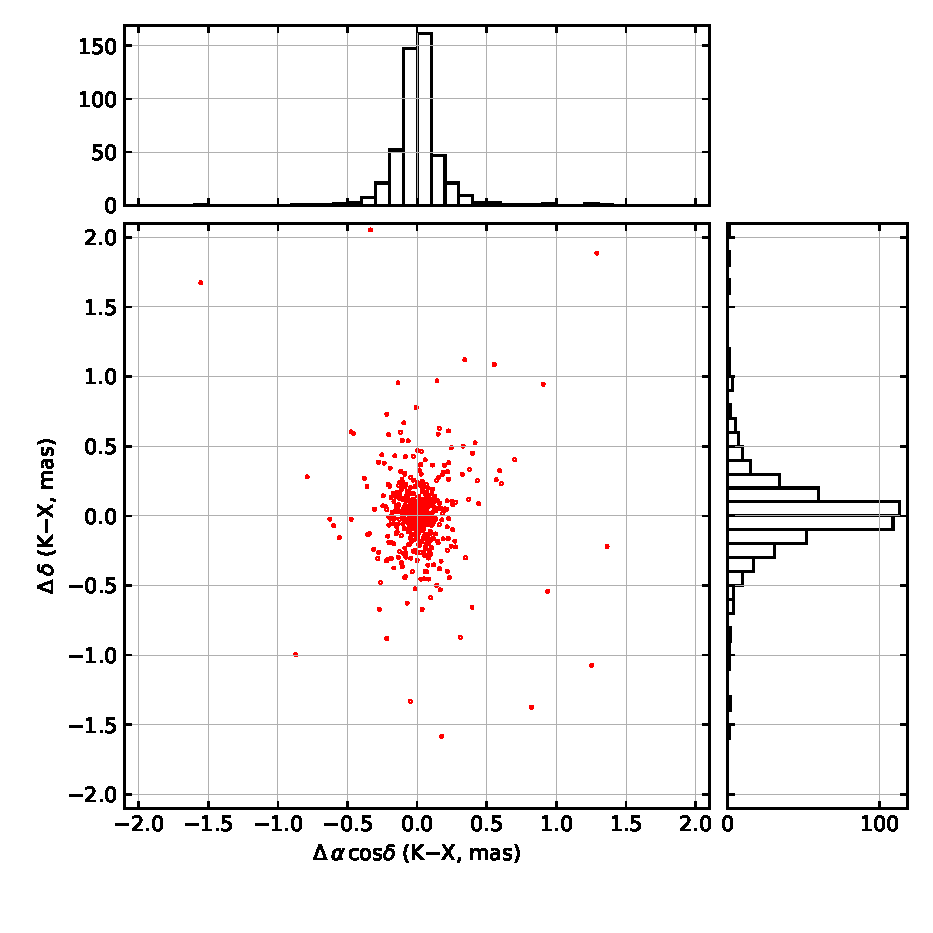
\includegraphics[width=60mm]{figs/k-sx-scatter}
        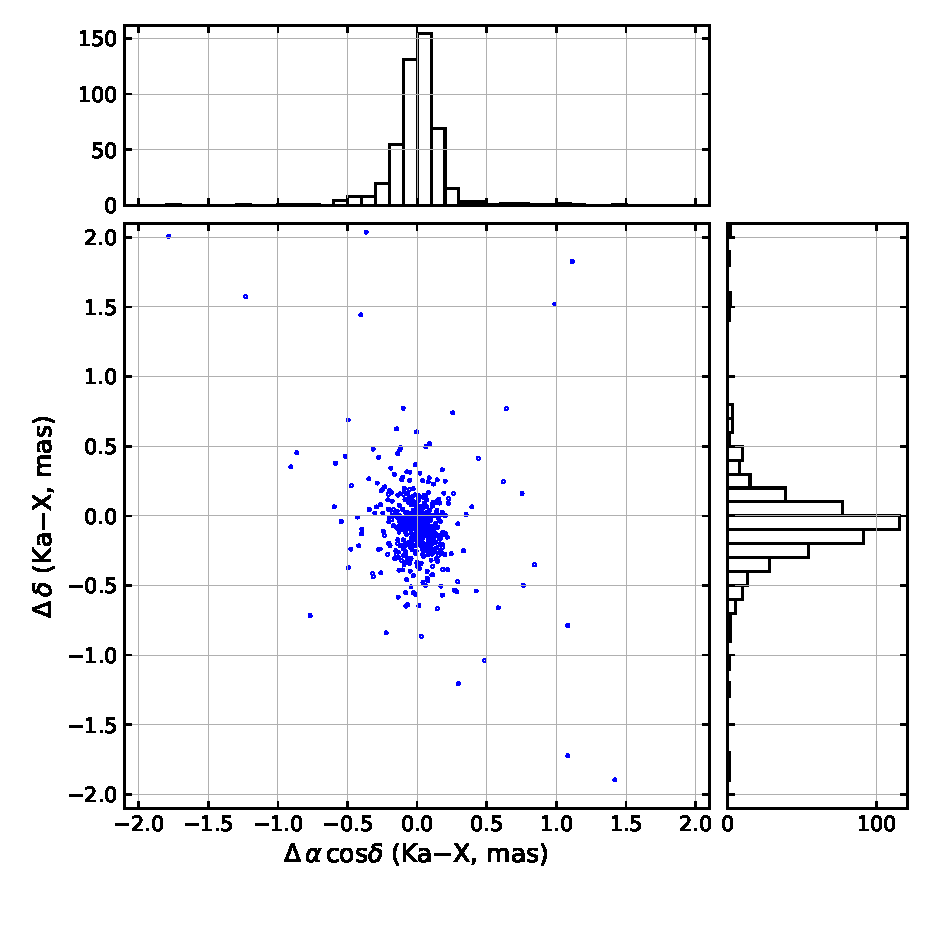
\includegraphics[width=60mm]{figs/xka-sx-scatter}
        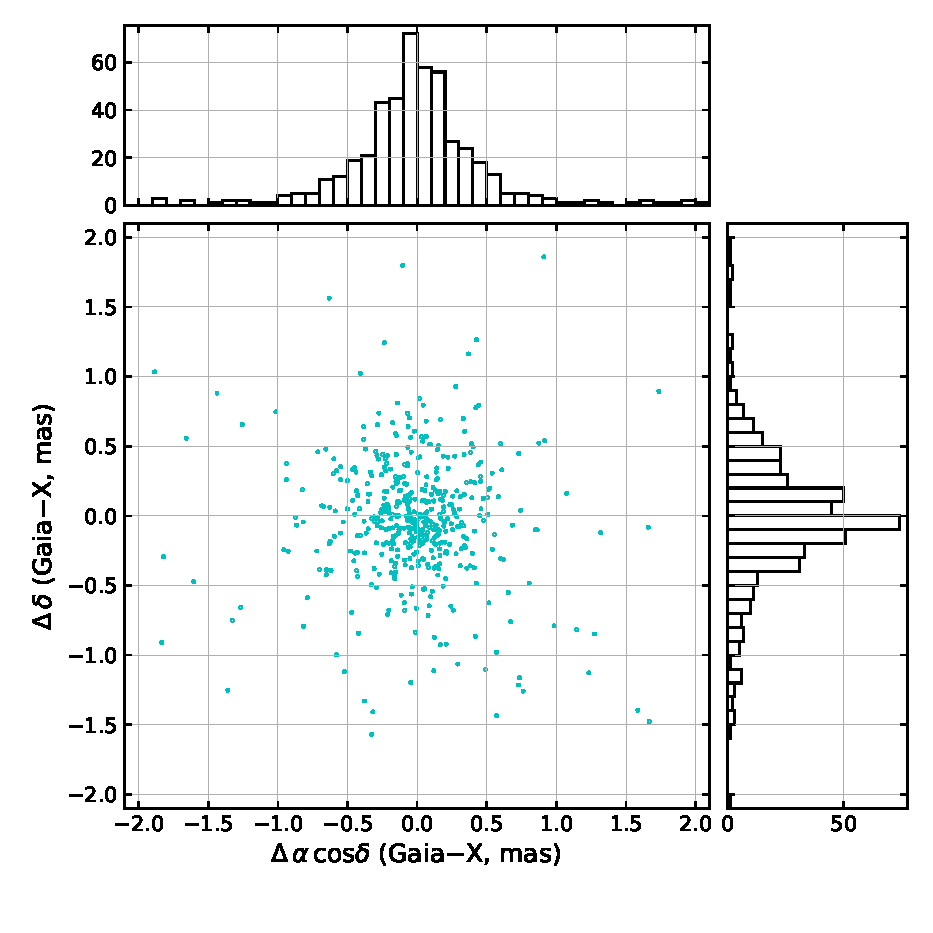
\includegraphics[width=60mm]{figs/gaia-sx-scatter}
        \caption[]{\label{fig:pos-offset-scatter}
            Position offset scatter and distribution of their components in the right ascension and declination for 488 sources of  $K$-band (top), $Ka$-band (middle) , and \textit{Gaia} (bottom) positions with respective to the $X$-band position after removing the global differences.
        }
    \end{figure}

   Table~\ref{tab:vsh01}-\ref{tab:vsh02} reports the VSH parameters of the first and second degrees, respectively.
   The transformation parameters between $K$-band and $X$-band positions are no greater than $30\,\mathrm{\mu as}$ except for $D_3$, $M_{20}$, and $E_{21}^I$.
   Similar results could be found between $Ka$-band and $X$-band; however, significant terms, $D_3$, $E_{20}$, and $M_{20}$ exceeding 0.3~mas are also reported, leading to a possible declination bias on the sub-mas level.
   %This result justifies the necessity of removing the global difference and aligning the celestial frames at other wavelengths to the $X$-band frame before analyzing of position offsets.
   Most of the transformation parameters between \textit{Gaia} and $X$-band range from $30\,\mathrm{\mu as}$ to $50\,\mathrm{\mu as}$.

   Figure~\ref{fig:pos-offset-scatter} presents the position offset scatters of $K$-band, $Ka$-band, and \textit{Gaia} positions relative to the $X$-band position, as well as distributions of their right ascension and declination components, for 488 common sources.
   The agreement between $K$-band and $X$-band positions is around 0.1~mas on the right ascension;
   the declination scatter is slightly larger, making the scatter cloud elongating along the declination axis.
   This phenomenon is more pronounced between $Ka$-band and $X$-band.
   The distribution of offset between \textit{Gaia} and $X$-band positions, with a nearly circle-like shape, is flatter than the $K$- and $Ka$-band, showing similar agreements of 0.3--0.5~mas on the right ascension and declination.
   No bias larger than 0.1~mas in neither right ascension nor declination could be observed for all three position offsets.
   Hence, we freed studies of multi-wavelength positions carried out in the next sections from large-scale differences. %due to deformations and alignment issues.
%
%______________________________________________________________

\subsection{Distribution of radio-to-optical offsets}    \label{subsec:r2o-dist}

%__________________________________________________  {fig:rho-hist}
    \begin{figure}[hbtp]
        \centering
        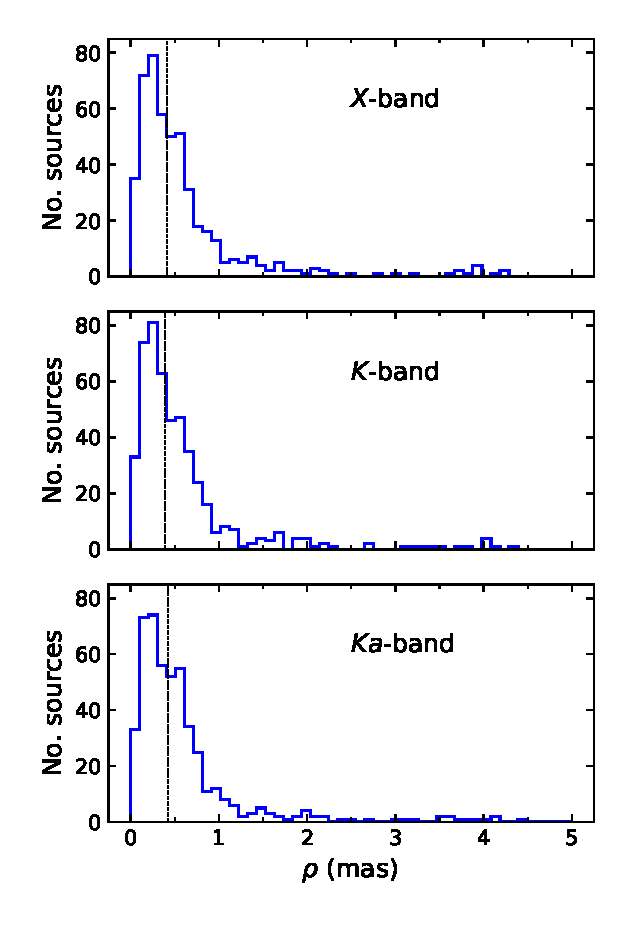
\includegraphics[width=0.45\columnwidth]{figs/rho-hist}
        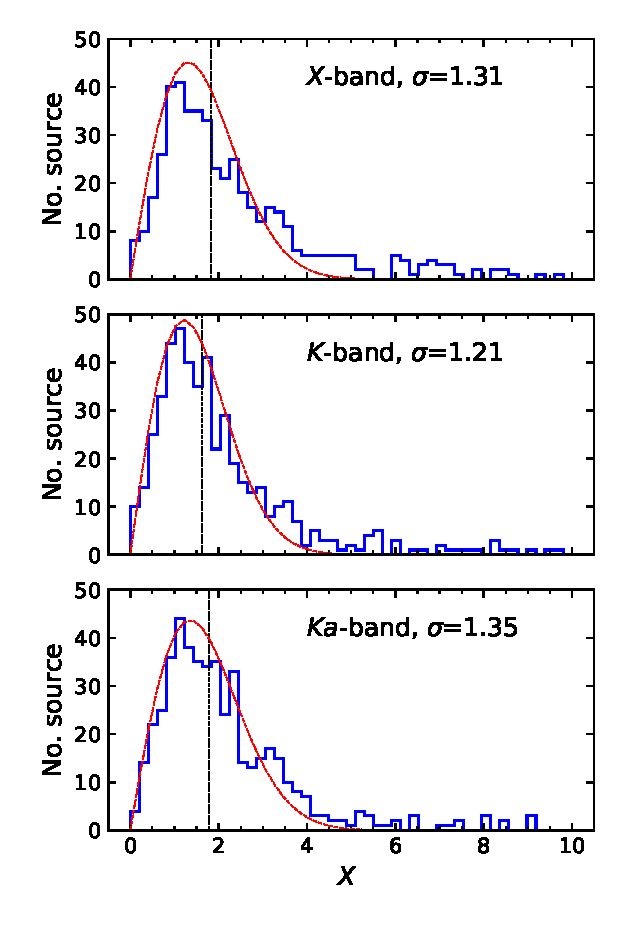
\includegraphics[width=0.45\columnwidth]{figs/X-hist}
        \caption[]{\label{fig:rho-hist}
            Distributions of radio-to-optical offset $\rho$ (left) and normalized separation $X$ (right) at $X$-, $K$-, and $Ka$-band for 488 sources.
            The red dashed curves represent fitted standard Rayleigh distributions based on sources with $X<X_0$ while the dark dashed line indicates the median value of each distribution.
        }
    \end{figure}

    Figure~\ref{fig:rho-hist} depicts the distributions of radio-to-optical offsets at $X$-, $K$-, and $Ka$-band, yielding similar shapes with median values of 0.41~mas, 0.40~mas, and 0.42~mas, accordingly.
    The 5th and 95th percentiles are 0.08~mas and 2.06~mas at $X$-band; 0.09~mas and 2.01~mas at $K$-band; and 0.09~mas and 2.16~mas at $Ka$-band.
    Only six sources have a radio-to-optical offset larger than 5~mas at either radio bands.
    We found a second peak at around 0.6~mas at all three bands, which is sharpest at the $X$-band.

    The distributions of normalized separations are slightly different: it is sharper for the $Ka$-band but flatter for the $X$-band (right panel in Fig.~\ref{fig:rho-hist}).
    There are 16 sources at $X$-band, 6 at $K$-band, and 8 at $Ka$-band with $X>10$, which are beyond the axis.
    For ideal cases, $X$ is supposed to follow a Rayleigh distribution of unit standard deviation, then the median value of $X$ would be 1.18.
    For a sample of $N$ sources, the number of sources with $X>X_0$ is expected to be less than one when $X_0=\sqrt{2\log{N}}$.
    For our sample ($N=488$), $X_0$ is 3.52.
    Medians of normalized separations are 1.89, 1.69, and 1.77 for $X$-, $K$-, and $Ka$-band, respectively, all greater than the predicted median value of ideal cases.
    We fitted the normalized separation distributions to the Rayleigh curve with an unknown standard deviation $\sigma$.
    The fitting returns the estimation of $\sigma$ to be 4.01 for $X$-band, 3.16 for $K$-band, and 3.22 for $Ka$-band.
    The distribution of $X$ would become much closer to the unit-standard-deviation Rayleigh shape ($\sigma \simeq 1.3$) if restricting sources to those with $X<X_0$.
    This criterion would rule out sources with statistically significant radio-to-optical offsets as outliers, whose number is 99 for $X$-band, 64 for $K$-band, and 66 for $K$-band, respectively.

    We further compared three radio-to-optical offsets of individual sources. %, as presented in Fig~\ref{fig:rho-vs-si}.
    Except for a few cases, the radio-to-optical offsets determined from $X$-, $K$-, and $Ka$-band are approximately equal.
    No statistically obvious evidence from our sample shows that the radio-to-optical offset decreases at high frequency.
    Further examinations report that the absolute difference among three radio-to-optical offsets for 95\% sources is less than 0.54~mas, which could be considered as an upper limit of the deviation among three radio-to-optical offsets for our sample.
    We observed similar results for normalized separations, regardless of the normalized separation at $X$-band is slightly larger than the other two bands.
%__________________________________________________

\subsection{Correlation between radio-to-optical offsets and source properties}    \label{subsec:r2o-corr}
%%
%__________________________________________________{fig:rho-g-mag}

    \begin{figure*}[hbtp]
        \centering
        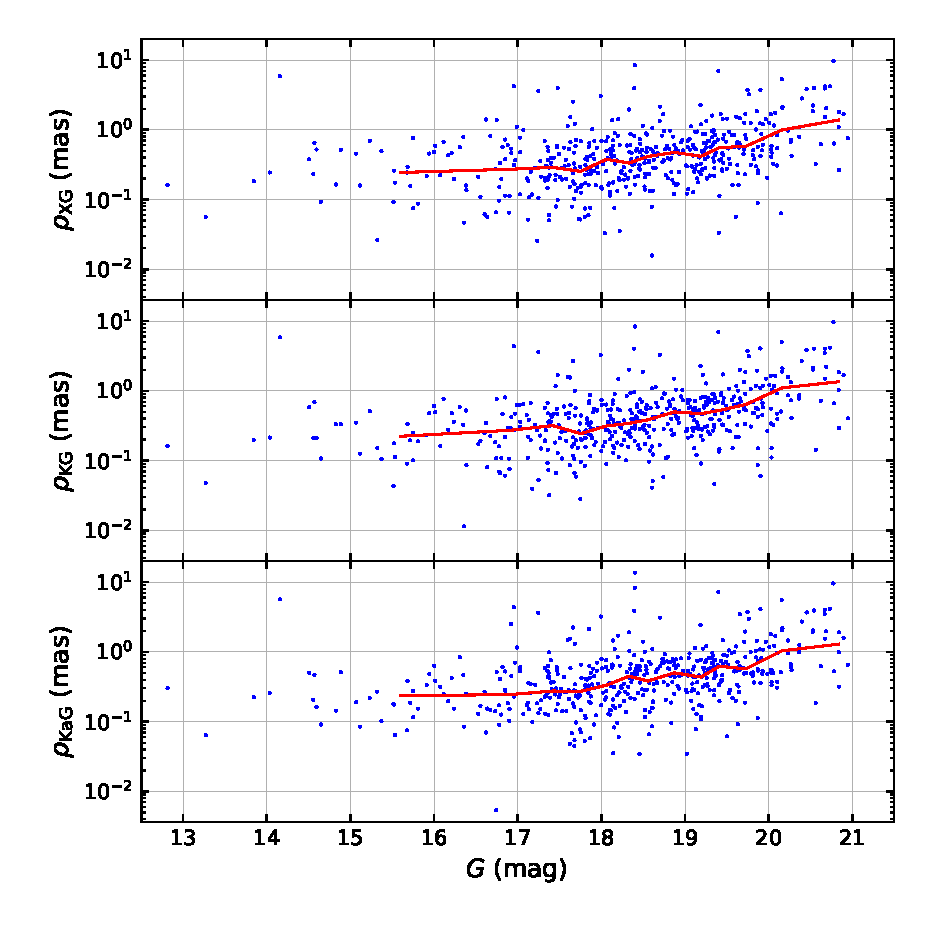
\includegraphics[width=0.7\columnwidth]{figs/rho-g-mag}
        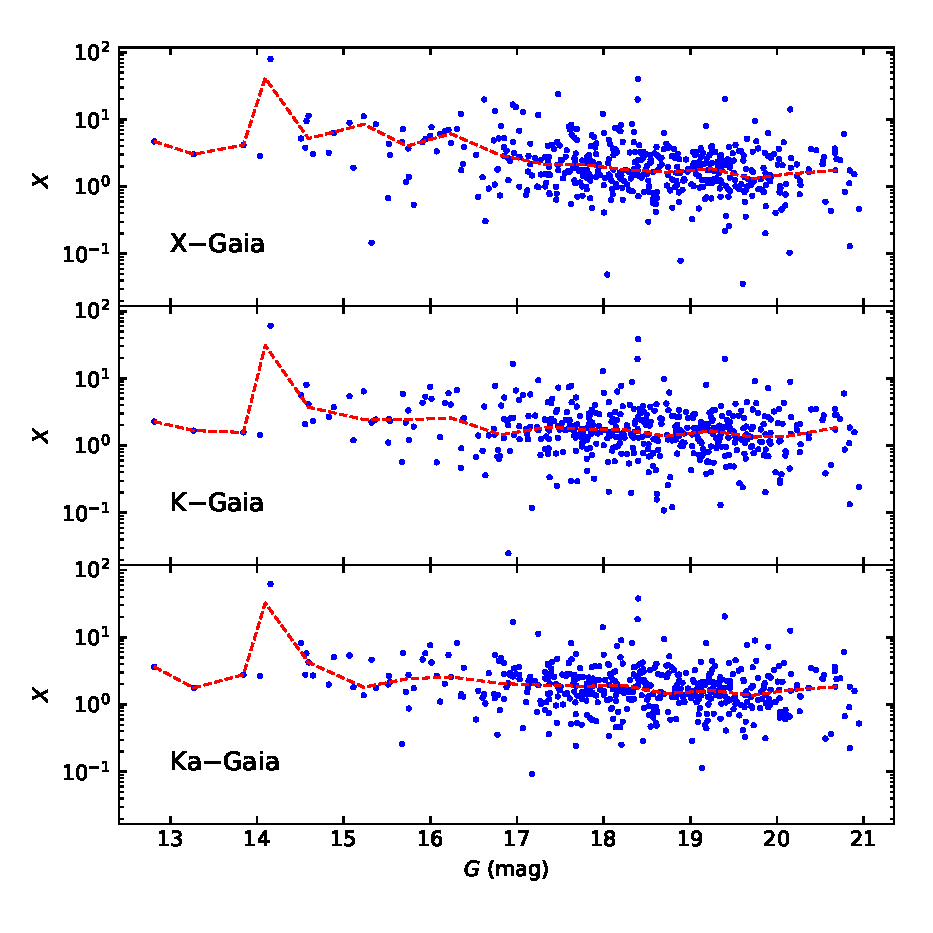
\includegraphics[width=0.7\columnwidth]{figs/X-g-mag}
        \caption[]{\label{fig:rho-g-mag}
            Radio-to-optical offsets (left) and normalized separations (right) at $X$-, $K$-, and $Ka$-band as a function of \textit{Gaia} $G$ magnitude for 488 sources.
            The red curve indicates the median value of every 40 sources.
        }
    \end{figure*}

%%
%__________________________________________________{fig:rho-vs-si}
    \begin{figure*}[hbtp]
        \centering
        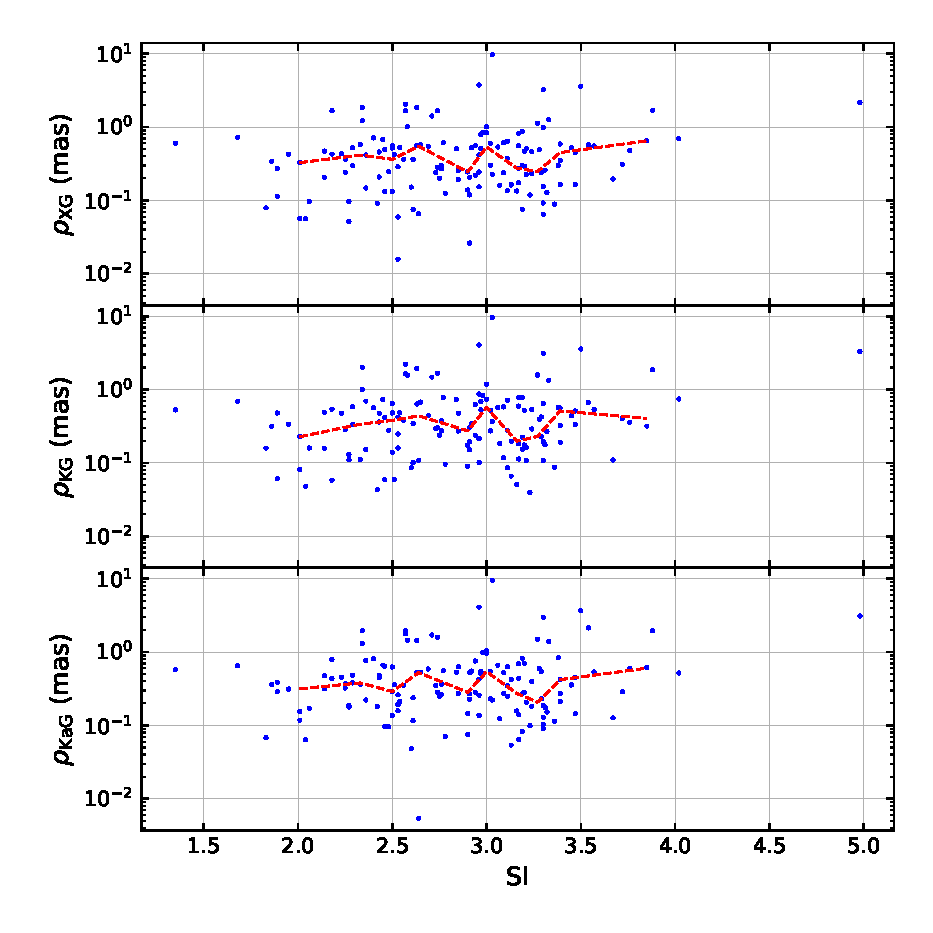
\includegraphics[width=0.4\columnwidth]{figs/rho-si}
        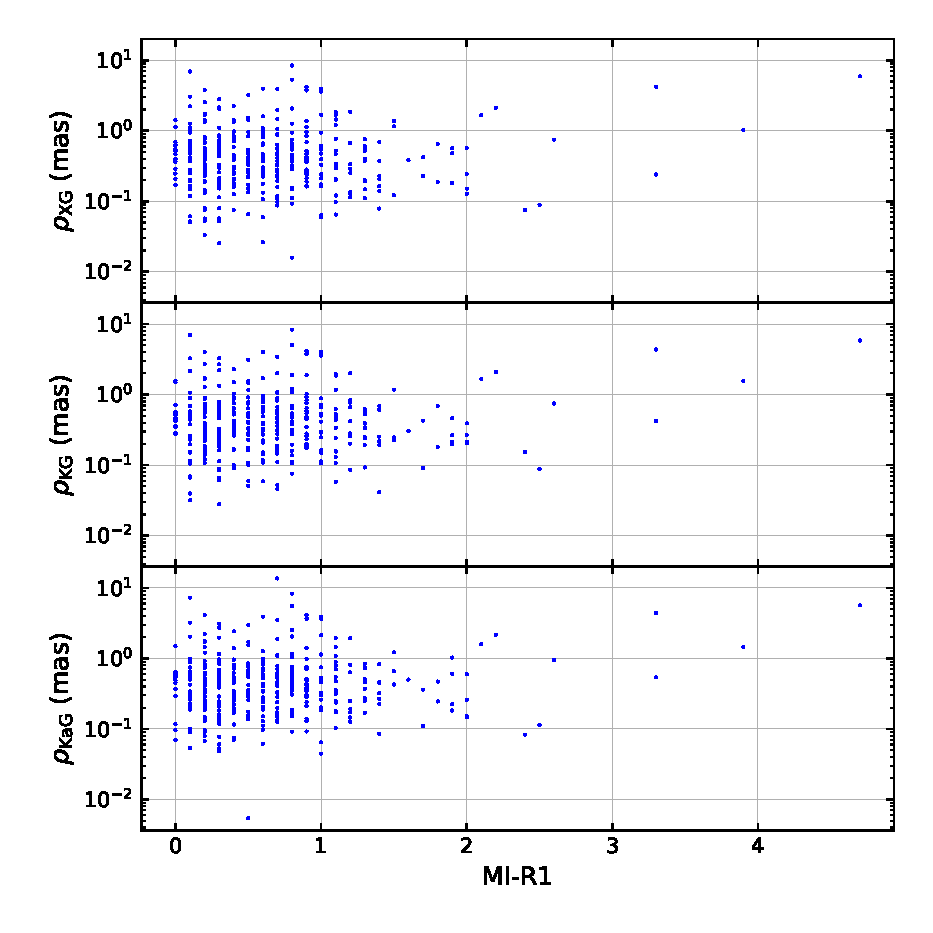
\includegraphics[width=0.4\columnwidth]{figs/rho-I1R}
        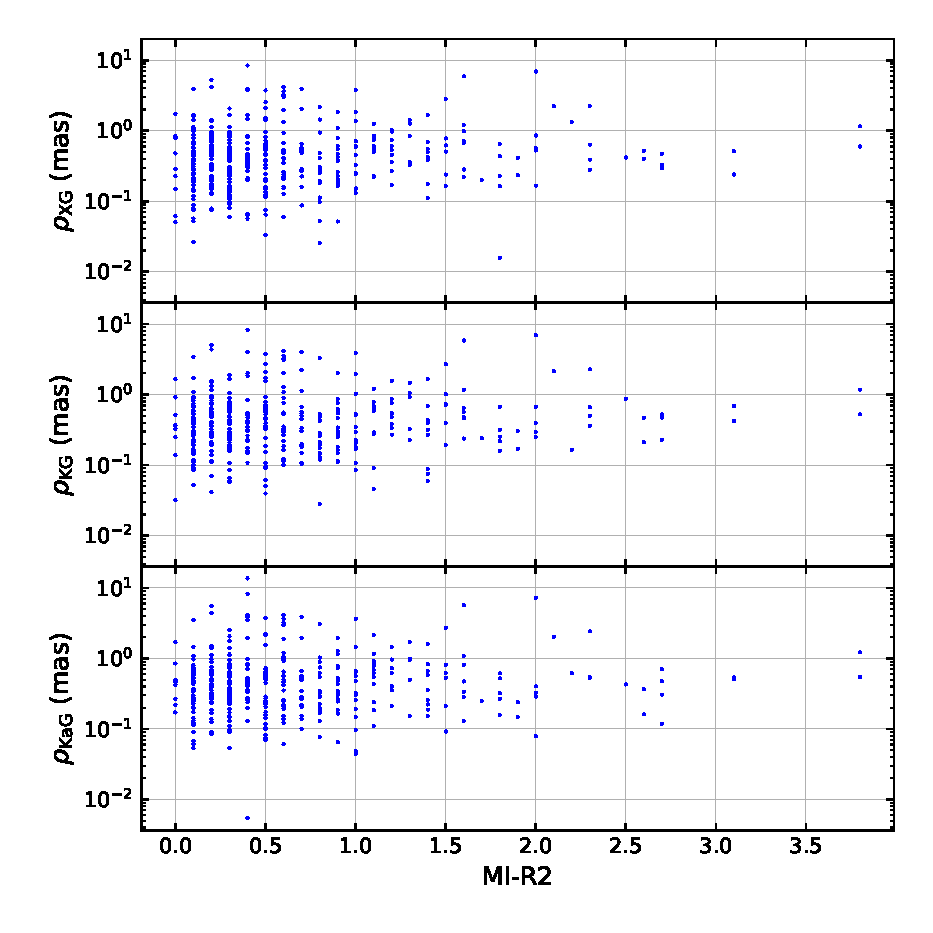
\includegraphics[width=0.4\columnwidth]{figs/rho-I2R}
        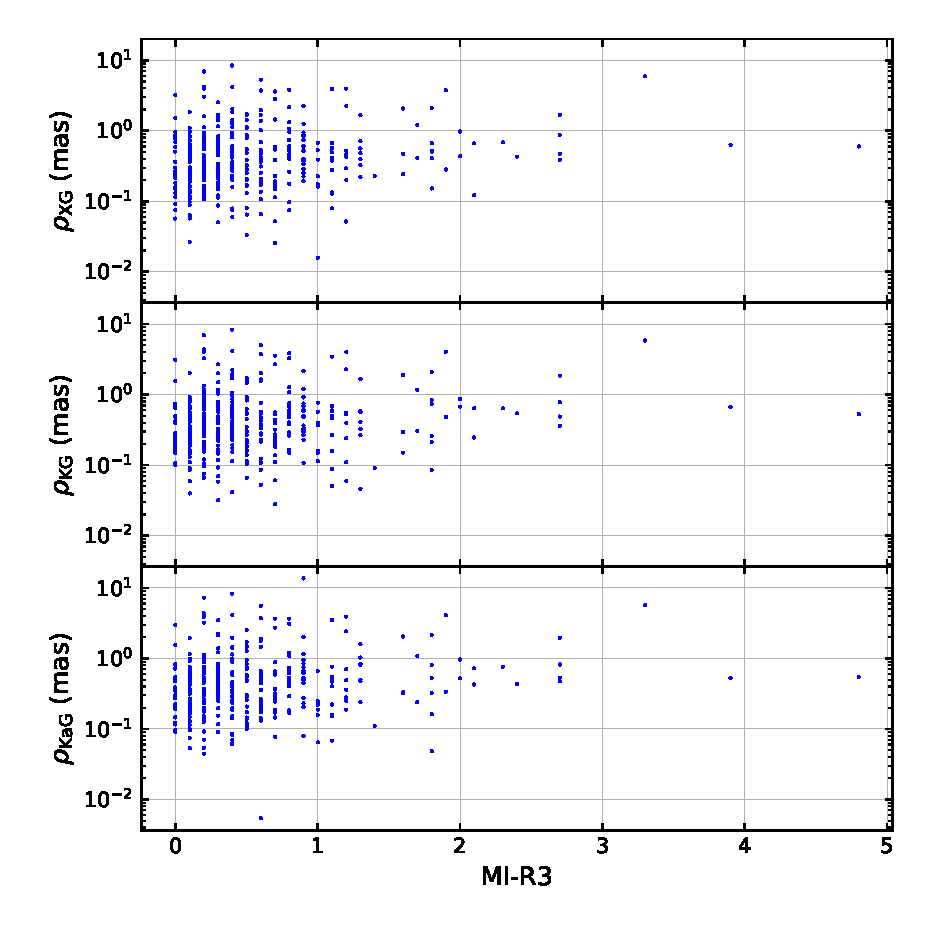
\includegraphics[width=0.4\columnwidth]{figs/rho-I3R}
%        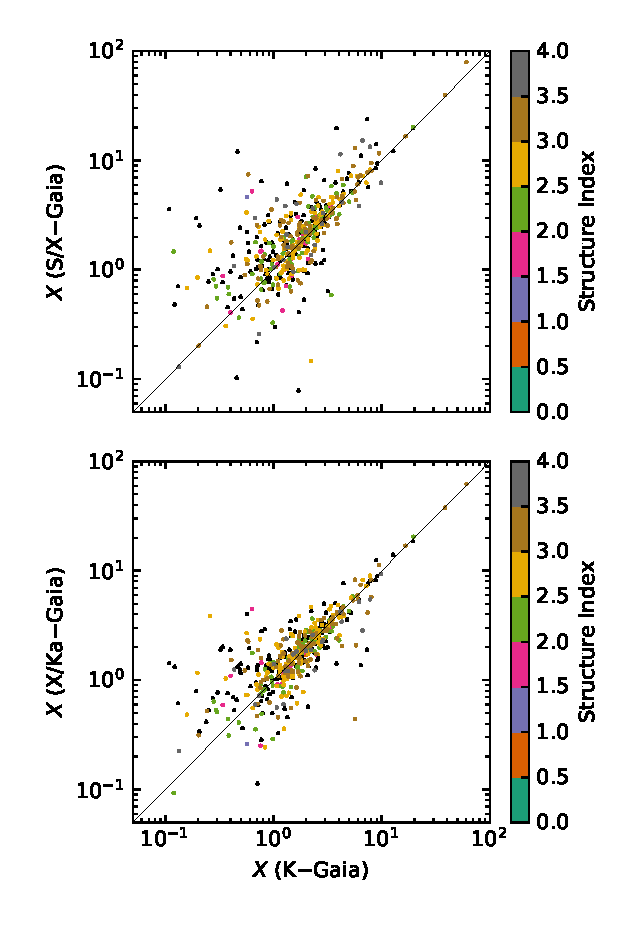
\includegraphics[width=80mm]{figs/X-com-vs-si}
        \caption[]{\label{fig:rho-vs-si}
            Radio-to-optical offsets at $X$-, $K$-, and $Ka$-band as a function of source structure index  (upper left) for 142 sources, and
            morphological SHARP (upper right), SROUND (lower left), and GROUND (lower right) indices from the R-filter image for 396 sources.
            The red curve indicates the median value of small bins.
            The bin size is set as 15 for the structure index.
        }
    \end{figure*}

%%
%__________________________________________________{fig:rho-z}

    \begin{figure}[hbtp]
        \centering
        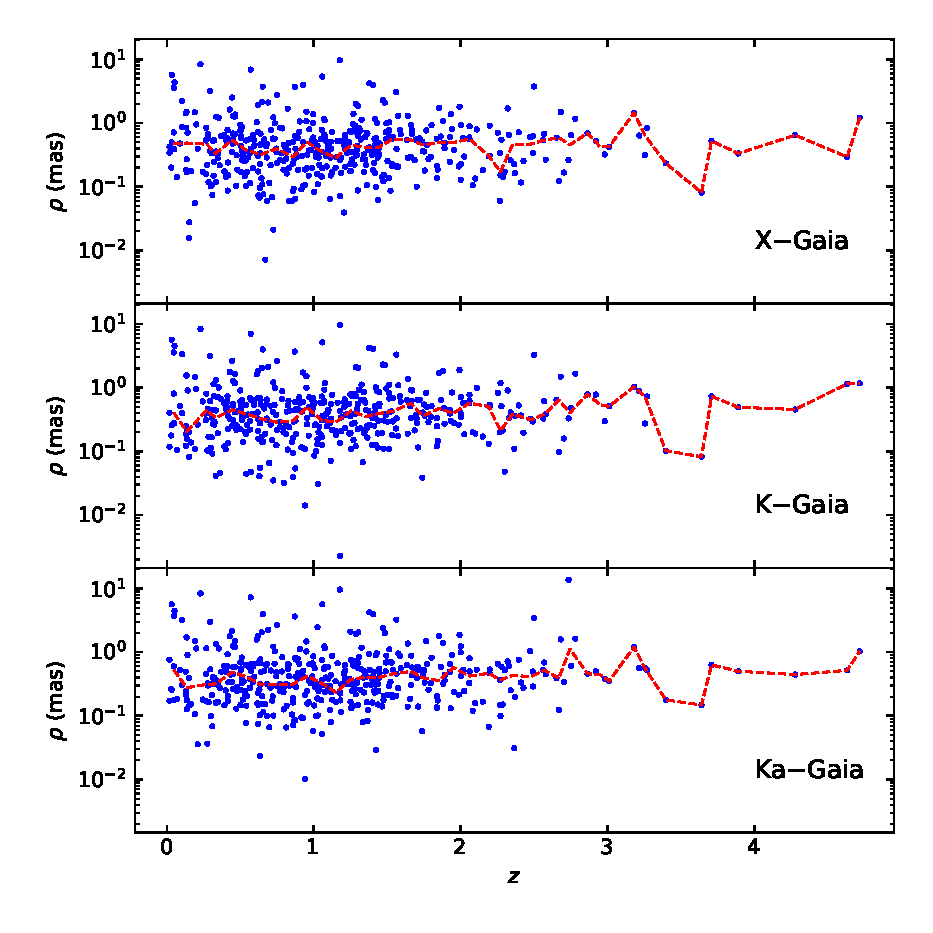
\includegraphics[width=0.7\columnwidth]{figs/rho-z}
        \caption[]{\label{fig:rho-z}
            Radio-to-optical offsets at $X$-, $K$-, and $Ka$-band as a function of red-shift $z$ for 443 sources having a red-shift measurements in the LQAC-5 catalog.
            The red curve indicates the median value of every 15 sources.
        }
    \end{figure}

    % Solution &No. Sessions   &No.Observations    &Postfit rms &Reduced $\chi^2$
    % &\multicolumn{2}{c}{Median error [$\mathrm{\mu as}$]}\\
    % \cmidrule(lr){6-7}
    %           &  &(delays)  &ps &
    %             &$\alpha\cos\delta$  &$\delta$  \\

%__________________________________________________
    \begin{table*}
        \centering
        \caption{\label{tab:corr_test}
            Correlation statistics between the radio-to-optical offsets and source properties for 488 sources used in this work.
        }
        \begin{tabular}{cccccccccc}
        \hline \noalign{\smallskip}
            &\multicolumn{3}{c}{$X$-band}  &\multicolumn{3}{c}{$K$-band}  &\multicolumn{3}{c}{$Ka$-band}  \\
            \cmidrule(lr){2-4}  \cmidrule(lr){5-7}  \cmidrule(lr){8-10}
            &$r$  &$rs$  &$\tau$  &$r$  &$rs$  &$\tau$  &$r$  &$rs$  &$\tau$  \\
        \noalign{\smallskip}
        \hline
        \noalign{\smallskip}
          $G$  &$+0.8$  &$+1.0$  &$+0.9$  &$+0.8$  &$+1.0$  &$+0.9$  &$+0.8$  &$+1.0$  &$+0.9$  \\
               &\textit{$8 \times 10^{-4}$}  &\textit{$3 \times 10^{-8}$}  &\textit{$6 \times 10^{-7}$}
               &\textit{$5 \times 10^{-4}$}  &\textit{$8 \times 10^{-8}$}  &\textit{$6 \times 10^{-7}$}
               &\textit{$3 \times 10^{-4}$}  &\textit{$2 \times 10^{-7}$}  &\textit{$2 \times 10^{-6}$}  \\
           SI  &$+0.3$  &$+0.2$  &$+0.2$  &$+0.2$  &$+0.3$  &$+0.2$  &$+0.3$  &$+0.2$  &$+0.1$  \\
               &\textit{0.37}  &\textit{0.56}  &\textit{0.60}  &\textit{0.51}  &\textit{0.47}  &\textit{0.48}  &\textit{0.36}  &\textit{0.68}  &\textit{0.86}  \\
        MI-B1  &$+0.2$  &$+0.0$  &$-0.0$  &$-0.4$  &$-0.4$  &$-0.3$  &$-0.3$  &$-0.4$  &$-0.3$  \\
               &\textit{0.60}  &\textit{0.99}  &\textit{1.00}  &\textit{0.27}  &\textit{0.23}  &\textit{0.22}  &\textit{0.39}  &\textit{0.21}  &\textit{0.29}  \\
        MI-B2  &$+0.2$  &$+0.4$  &$+0.3$  &$+0.5$  &$+0.5$  &$+0.4$  &$+0.4$  &$+0.5$  &$+0.3$  \\
               &\textit{0.49}  &\textit{0.27}  &\textit{0.28}  &\textit{0.18}  &\textit{0.11}  &\textit{0.15}  &\textit{0.25}  &\textit{0.17}  &\textit{0.21}  \\
        MI-B3  &$-0.6$  &$-0.7$  &$-0.6$  &$+0.1$  &$-0.2$  &$-0.2$  &$+0.1$  &$-0.2$  &$-0.2$  \\
               &\textit{0.06}  &\textit{0.01}  &\textit{0.02}  &\textit{0.79}  &\textit{0.54}  &\textit{0.42}  &\textit{0.69}  &\textit{0.51}  &\textit{0.42}  \\
        MI-R1  &$-0.6$  &$-0.4$  &$-0.3$  &$-0.2$  &$-0.1$  &$-0.0$  &$+0.2$  &$+0.1$  &$+0.1$  \\
               &\textit{0.10}  &\textit{0.28}  &\textit{0.29}  &\textit{0.52}  &\textit{0.83}  &\textit{1.00}  &\textit{0.65}  &\textit{0.85}  &\textit{0.73}  \\
        MI-R2  &$+0.5$  &$+0.2$  &$+0.1$  &$+0.4$  &$+0.3$  &$+0.2$  &$+0.3$  &$-0.0$  &$-0.1$  \\
               &\textit{0.18}  &\textit{0.58}  &\textit{0.59}  &\textit{0.26}  &\textit{0.35}  &\textit{0.37}  &\textit{0.33}  &\textit{0.89}  &\textit{0.59}  \\
        MI-R3  &$+0.7$  &$+0.7$  &$+0.6$  &$+0.7$  &$+0.8$  &$+0.6$  &$+0.7$  &$+0.7$  &$+0.6$  \\
               &\textit{0.02}  &\textit{0.02}  &\textit{0.02}  &\textit{0.03}  &\textit{0.01}  &\textit{0.01}  &\textit{0.03}  &\textit{0.02}  &\textit{0.01}  \\
       MI-IR1  &$-0.1$  &$-0.1$  &$-0.1$  &$-0.3$  &$+0.2$  &$+0.1$  &$-0.2$  &$+0.1$  &$+0.1$  \\
               &\textit{0.86}  &\textit{0.66}  &\textit{0.64}  &\textit{0.40}  &\textit{0.60}  &\textit{0.64}  &\textit{0.51}  &\textit{0.65}  &\textit{0.74}  \\
       MI-IR2  &$+0.1$  &$+0.1$  &$+0.1$  &$+0.1$  &$+0.1$  &$-0.0$  &$+0.5$  &$+0.5$  &$+0.4$  \\
               &\textit{0.65}  &\textit{0.72}  &\textit{0.63}  &\textit{0.66}  &\textit{0.70}  &\textit{0.95}  &\textit{0.07}  &\textit{0.11}  &\textit{0.09}  \\
       MI-IR3  &$+0.4$  &$+0.2$  &$+0.1$  &$+0.6$  &$+0.3$  &$+0.2$  &$+0.5$  &$+0.4$  &$+0.3$  \\
               &\textit{0.22}  &\textit{0.49}  &\textit{0.63}  &\textit{0.06}  &\textit{0.31}  &\textit{0.30}  &\textit{0.08}  &\textit{0.15}  &\textit{0.19}  \\
       $z$  &$+0.7$  &$+0.3$  &$+0.3$  &$+0.9$  &$+0.5$  &$+0.4$  &$+0.8$  &$+0.8$  &$+0.6$  \\
            &\textit{$6 \times 10^{-3}$}  &\textit{0.27}  &\textit{0.25}  &\textit{$4 \times 10^{-4}$}
            &\textit{0.11}  &\textit{0.12}  &\textit{$2 \times 10^{-3}$}  &\textit{$5 \times 10^{-3}$}  &\textit{$5 \times 10^{-3}$}  \\
       \hline \noalign{\smallskip}
       %-- X vs G
       $G$  &$-0.8$  &$-0.7$  &$-0.6$  &$-0.8$  &$-0.7$  &$-0.6$  &$-0.9$  &$-0.8$  &$-0.6$  \\
            &\textit{$2 \times 10^{-3}$}  &\textit{$6 \times 10^{-3}$}  &\textit{$7 \times 10^{-3}$}
            &\textit{$5 \times 10^{-4}$}  &\textit{$5 \times 10^{-3}$}  &\textit{$4 \times 10^{-3}$}
            &\textit{$2 \times 10^{-4}$}  &\textit{$2 \times 10^{-3}$}  &\textit{$2 \times 10^{-3}$}  \\
       \hline \noalign{\smallskip}
       \end{tabular}
       \tablefoot{
        The Pearson, Spearman, and Kendall correlation coefficients are represented by $r$, $rs$, and $\tau$, respectively.
        The p-value of each statistical test is given in italics right below the correlation coefficient.
        A lower p-value suggests a more confident correlation.
        The last row gives the correlation between normalized separation $X$ and $G$-mag.
        The data were binned before the statistical tests.
       }
   \end{table*}

%
    Figure~\ref{fig:rho-g-mag} demonstrates a correlation between the radio-to-optical offsets and \textit{Gaia} $G$ magnitude: the radio-to-optical offsets increase towards the faint end for all three radio bands.
    This correlation could be still seen if we included all the common sources between each ICRF catalog and \textit{Gaia}-CRF2 subsets, for instance, the 2820 sources between the ICRF3 $X$-band catalog and \textit{Gaia}-CRF2.

    We found 142 matches with the structure index information available.
    For most sources, the structure index falls in the range of 2 to 3.5.
    The radio-to-optical offsets against the structure index ars plotted in the upper left panel of Fig.~\ref{fig:rho-vs-si}, where we could not observe an obvious correlation.

    In our sample of 488 common sources, 199 sources associated with the morphological index at the filter $B$, 396 at the filter $R$, and 340 at the filter $IR$.
    All three morphological indices larger than one was found for 9 sources at the filter $B$, 16 sources at the filter $R$, and 25 sources at the filter $IR$, corresponding to about 5\%, 4\%, and 7\% of the subset with these morphological indices available, respectively.
    Figure~\ref{fig:rho-vs-si} demonstrates a smooth dependency of the radio-to-optical distance on the three morphological indices of $R$-filter.
    The morphological index of filter $B$ and $IR$ present similar results to those of filter $R$ and thus are not plotted here.

    The redshift measurement is given for 443 sources.
    We did not see any dependency of neither radio-to-optical angular separation as shown in Fig.~\ref{fig:rho-z}.

     % nor normalized separation (not plotted for brevity) on the redshift.
     Then we performed correlation statistical tests between radio-to-optical offsets and properties parameters mentioned above.
     The statistical tests consisted of a parametric analysis on the Pearson correlation and two non-parametric analyses on the Spearman and Kendall correlations.
     In order to get robust results, we binned the sources and adopted the median values in the bins.
     The bin size was chosen to make sure that we had at least 10 bins.
     It was set as 40 for $G$ magnitude, $z$, and MI at filter $R$, 20 for MI at filter $B$, 30 for MI at filter $IR$, and 15 for SI.
     The curve of binned data is colored in red in Figs~\ref{fig:rho-g-mag}-\ref{fig:rho-z}.
     Table~\ref{tab:corr_test} summarizes the results of statistical tests.
     We considered all three correlation coefficients greater than 0.5 in the absolute sense with confidence levels higher than 99\% (p-value <0.1) as a genuine correlation.
     Therefore, we detected a positive correlation of the radio-to-optical offsets determined at all three radio bands with the $G$ magnitude, as already presented in Fig~\ref{fig:rho-g-mag}.
     Another positive correlation is found between the radio-to-optical offset and redshift at $Ka$-band but not at $X$- or $K$-band.

     We also plotted the normalized separation against the $G$ magnitude in Fig.~\ref{fig:rho-g-mag} and found a slightly decreasing trend for $X$-band and flat trends for $K$- and $Ka$-band at $17<G<20$.
     The statistical test (last row in Table~\ref{tab:corr_test}) suggested a negative correlation between the normalized separation and the $G$ magnitude.

%__________________________________________________

\subsection{Aligned multi-wavelength positions}    \label{subsec:pos-align}


    In this section, we used the direction information of the position offset to investigate the relation of multi-wavelength positions for individual sources.
    The position angles of $K$-band, $Ka$-band, and \textit{Gaia} positions with referred to the $X$-band position are plotted in Fig.~\ref{fig:pa-hist}.
    Peaks at around $0\,^\circ$, $180\,^\circ$, and $360\,^\circ$ could be observed for $K$- and $Ka$-band positions, while \textit{Gaia} position does not show a similar preference.

    In order to compare the position angles of $K$-band, $Ka$-band, and \textit{Gaia} positions with respect to the $X$-band position,
    we calculated the differences between these position angles and wrapped them into the range of ($-180^\circ$, $180^\circ$].
    Figure~\ref{fig:pa-diff} depicts the distribution of position angle differences, where one could observe a clear peak around $0^\circ$ while no peak appears at $\pm 180^\circ$.

    We performed a Monte-Carlo simulation to test if the peak around zero in Fig.~\ref{fig:pa-diff} was caused by chance.
    We created 10\,000 random permutations of the positions in each catalog, calculated the orientation (PA) of their position offset vectors and then computed the mean histogram and its standard deviation.
    This procedure was done between $K$- and $X$-band positions, between $Ka$- and $X$-band positions, and between \textit{Gaia} and $X$-band positions, separately.
    The mean histogram and the confident intervals of 66\%, 95\%, and 99\% are also shown in Fig~\ref{fig:pa-diff}.
    The confidence of the peak of the ``true'' data histogram is well above 99\%, making the alignment very significant.

    We empirically adopted a limit of $30^\circ$ on the absolute PA difference $|\Delta PA|$, below which the multi-wavelength positions could be considered as aligned.
    As a result, we obtained a sample of 55 sources having positions at four frequencies aligned.
    Among these sources, we found the jet direction measurement for 22 sources from \citet{2019ApJ...874...43L}.
    Figure~\ref{fig:jet-pa-com} depicts the distribution of the difference between the jet direction $PA_\mathrm{jet}$ and $X$-to-\textit{Gaia} orientation $PA_\mathrm{XG}$.
    The difference between $PA_\mathrm{jet}$ and $PA_\mathrm{XG}$ falling into the interval of ($-30^\circ$, $30^\circ$) happens to six sources,
    which are considered as having the radio-to-optical offset in the downstream of the jet in the following discussion.
    Similarly, seven sources with $150^\circ < |PA_\mathrm{jet} - PA_\mathrm{XG}| < 180^\circ$ are considered as the case that the radio-to-optical offset is in the upstream of the jet.
    We compared the position offset vectors with the radio image and found that the positions at four bands are usually located within the compact core (<0.5~mas) except for few cases.
    The positions offsets for 22 sources with four positions aligned are plotted in Figs.~\ref{fig:jet-down}-\ref{fig:other}.

%%
%__________________________________________________{fig:pa-hist}

    \begin{figure}[hbtp]
        \centering
        \includegraphics[width=0.7\columnwidth]{figs/pa-hist}
        \caption[]{\label{fig:pa-hist}
            Distributions of the position angle of offset vector of $K$-band, $Ka$-band, and \textit{Gaia} positions with referred to the $X$-band position for 488 common sources.
        }
    \end{figure}

%%
%__________________________________________________{fig:pa-diff}

    \begin{figure}[hbtp]
        \centering
        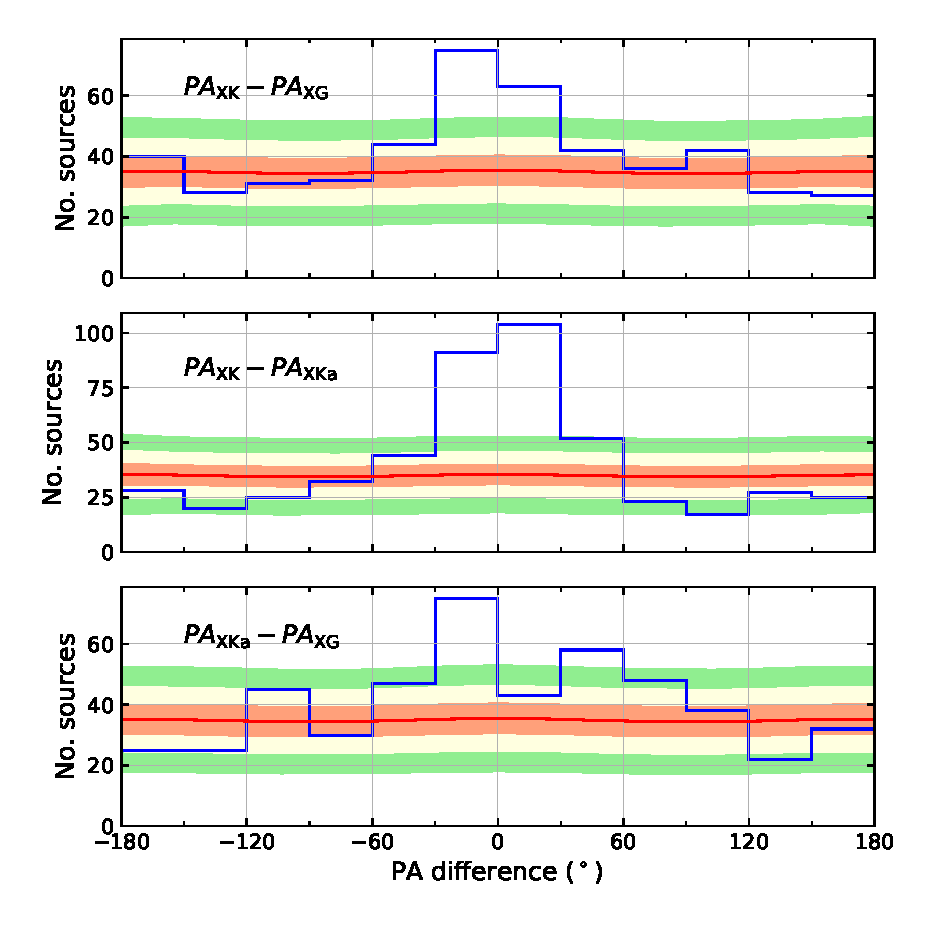
\includegraphics[width=0.7\columnwidth]{figs/pa-diff}
        \caption[]{\label{fig:pa-diff}
            Distributions of the position angle difference of offset vectors of $K$-band, $Ka$-band, and \textit{Gaia} positions with referred to the $X$-band position for 488 common sources.
%            The horizontal red dashed line stands for a uniform distribution.
            The red curve stands for mean histogram and shading zones represent the confidence intervals of 66\%, 95\%, and 99\% .
        }
    \end{figure}

%%
%__________________________________________________{fig:jet-pa-co}

    \begin{figure}[hbtp]
        \centering
        \includegraphics[width=0.7\columnwidth]{figs/jet-pa-com}
        \caption[]{\label{fig:jet-pa-com}
            Distribution of the position angle difference of $X$-to-\textit{Gaia} position offset vector and jet vector for 22 sources whose four-band positions are almost aligned ($|\Delta PA|~<~30^{\circ}$).
        }
    \end{figure}

%__________________________________________________

\section{Discussion} \label{subsec:discussion}
%
%__________________________________________________

\subsection{Cause of radio-to-optical distance} \label{subsec:cause-of-VG}
%
    \citet{2017MNRAS.471.3775P} summarize several causes for non-coincidence of the emission centers measured by the VLBI and \textit{Gaia}.
    They include:\\
    (1) large uncertainties in the \textit{Gaia} or/and VLBI positions;\\
    (2) optical structure (jet) at mas-scale; \\
    (3) optical position shift due to luminous host galaxy or asymmetry structure;\\
    (4) radio source structure and core-shift effect;\\
    (5) gravitational lensing and dual AGNs.\\
    We checked these items based on our results except the second one that has been studied deeply in \citet{2017A&A...598L...1K,2017MNRAS.467L..71P,2017MNRAS.471.3775P,2019MNRAS.482.3023P,2019ApJ...871..143P,2020MNRAS.493L..54K}. %, and the last one which happens for few cases.

    The \textit{Gaia} astrometric precision gets worse as one moves to the faint end, and this holds true for quasar positions \citep{2016A&A...595A...5M,2018A&A...616A..14G}, while VLBI formal error does not yield such a dependency.
    We observed that the radio-to-optical offsets increase slightly with the $G$-magnitude in the range of $17<G<21$, as presented in Fig.~\ref{fig:rho-g-mag}.
    It justifies the criterion of being optically bright for selecting suitable optical-to-radio frame-tie sources, e.g., in \citet{2008A&A...490..403B,2012MmSAI..83..952M}.
    However, the normalized separations between VLBI and \textit{Gaia} positions are flat over or even decrease with $G$ magnitude.
    These results suggest that the large offsets at the fainter end are accounted for by the \textit{Gaia} formal error, making them less significant.
    \citet{2020A&A...634A..28L} also suggest that the global accuracy of the \textit{Gaia}-CRF2 position does not degrade with increasing the limiting magnitude of the sample.
    Hence, the objects for the link between \textit{Gaia}-CRF and ICRF may not have to be optically bright.

    The radio source structure seen at low frequencies might shift the observed position at $X$-band while the $K$- and $Ka$-band positions are less affected.
    If the strong source structure exists in the most radio sources, the radio-to-optical distance would statistically decrease at higher frequencies.
    We did not observe such a tendency.
    Instead, the radio-to-optical offsets at different bands are roughly at the same level, with a deviation of <~0.54~mas for most sources.
    For individual sources, however, radio-to-optical offsets might be significantly inconsistent.
    For instance, for 1315--058 the radio-to-radio offsets at $X$- and $K$-band are around 0.3~mas, but at $Ka$-band it is as large as 13.6~mas.
    A possible explanation could be that \textit{Gaia} measures the position of the same radio component as the $K$- and $X$-band does, while the $Ka$-band measures another one.

	The correlation offset between ground-based optical position and VLBI position for ICRF sources is not consisent.
	For example, \citet{2011A&A...532A.115C,2014AJ....147...95Z} report that the radio-to-optical offset increases with the structure index,
	while \citet{2013MNRAS.430.2797A} do not detect any dependency.
    For our sample, the structure index for sources with a radio-to-optical distance larger than 1~mas mainly exceeds 2.5, suggesting that large radio-to-optical distance is usually associated with a large structure index.
    But a large structure index, in turn, does not always match a large radio-to-optical distance (>1~mas).
    In general, the radio-to-optical distances show no or negligible correlation with the structure index.

    Since there are only a few cases with larger morphological indices than one, the influence of the host galaxy on the \textit{Gaia} position, if exist, is not significant for the bulk of our sample.
    Note that these morphological indices were determined from the optical imaging with a resolution of arc-second level, they could not be used to probe the mas-scale optical jet.
    Morphological indices based on high-resolution images might be useful to infer the existence of the mas-scale optical jet found by \citet{2017MNRAS.467L..71P}.

    If all sources have an extended structure of a similar scale, the radio-to-optical offset would become less as moving far away from us.
    It means that the radio-to-optical offset will decrease with the redshift, that is, the radio-to-optical offset is positively correlated with the redshift.
    This kind of correlation is found in \citet{2014AJ....147...95Z} but not in \citet{2013A&A...553A..13O}.
    However, we found a positive correlation between radio-to-optical offset at $Ka$-band with the redshift at a confidence of 99\%.
    This result is hard to explain at this moment and thus should be re-examined with future $Ka$-band solutions.
    \citet{2017ApJ...835L..30M} find that the radio-to-optical distance becomes significant at $z<0.5$.
    They infer that the shift of \textit{Gaia} position due to the extend optical structure effect explains partly the significant radio-to-optical distance, and this effect would become smaller for distant sources
    % The radio-to-optical distance does not correlate with the redshift as seen from our sample (Fig.~\ref{fig:rho-z}).
    At the interval of $z<0.5$, the number of sources becomes sparse, preventing us from drawing any conclusion within this range.

%__________________________________________________

\subsection{Frequency-position relation} \label{subsec:freq-pos}

    The preferred angle in Fig.~\ref{fig:pa-diff} is zero while no peak shows up at 180 degrees, indicating that the $K$-band, $Ka$-band, and \textit{Gaia} positions prefer being on the same side of the $X$-band position.
    This result differs from that expected from the north-south systematics in $K$- and $Ka$-band frame with respect to the $X$-band and \textit{Gaia} frames as shown in Fig.~\ref{fig:pa-hist}.
    The simulation results also support that the peak at $0^{\circ}$ is genuine rather than a chance peak.

    We found 55 sources, about 10\% of the sample, showing roughly aligned positions within $30~^\circ$ at four frequencies.
    Among these sources, 13 out of 22 sources ($>50\%$) with available jet direction information have the radio-to-optical vector parallel to the jet (upstream or downstream).
    If this result holds true for a large sample, it might serve as an astrometric method of determining the jet direction.

    From a simple core-jet model, the optical emission is at the base of the jet while radio cores are shifted along with the jet.
    Therefore, we could predict that the dominant scheme of the source positions is, staring from jet upstream, \textit{Gaia} position coming first (closest to the black hole), followed by the $Ka$-, $K$-, and $X$-band position.
    For seven sources whose four positions are aligned with the \textit{Gaia} position in the jet upstream, their multi-wavelength positions do not follow this scheme.
    We also note that on the full sample, most of the sources are not aligned.
    As a result, the multi-wavelength comparison suggests that the gross population of the radio sources is not following a simple core-jet model but possibly more complex systems like multi-black holes or various components emitting at different wavelengths.

%__________________________________________________

\subsection{Influence from the large-scale difference} \label{subsec:sys-effect}

    Our previous work reports that the global differences amongst ICRF3 and \textit{Gaia}-CRF2 catalogs would bias the radio-to-optical offset studies \citep{2020A&A...634A..28L}.
    Therefore, we removed the global difference of $K$-band, $Ka$-band, and \textit{Gaia}-CRF2 frames relative to the $X$-band frame.
    If this procedure is omitted, we would find a declination bias $\sim-0.3~{\rm mas}$ in the $Ka$-to-$X$ position offset, while $K$-to-$X$ and \textit{Gaia}-to-$X$ offsets are less affected.
    The peaks around $180^\circ$ in the position angle of $K$-to-$X$ and $Ka$-to-$X$ offset shown in Fig~\ref{fig:pa-diff} would be more pronounced, while the peaks at $0^\circ$ of position angle difference would be biased.
    On one hand, it indicates that such an alignment relation amongst four-frequency positions is sensitive to the global systematics.
    On the other hand, this result also justifies the reliability of the ICRF3 $X$-band frame, otherwise, the alignment might be biased by the frame deformation in the $X$-band frame.

%______________________________________________________________

\section{Conclusions} \label{sec:conclusions}

   We compared the positions of 488 extragalactic sources at radio $X$-, $K$-, $Ka$-band from the ICRF3 catalog and the optical position from the \textit{Gaia}-CRF2 subset to study the frequency-position relation, especially the radio-to-optical offset.
   We found:
   %
   \begin{enumerate}
   \item Radio-to-optical distance is at the same level estimated (difference less than 0.5~mas) at $X$-, $K$-, and $Ka$-band for 90\% of the sample.
   % There are 44 sources show good agreements among three radio positions but large radio-to-optical offsets.
   % For few cases, the \textit{Gaia} position matches radio positions of only two bands.
   \item Large radio-to-optical distances ($>1\,{\rm mas}$) are usually associated with a large source structure index ($>3$).
   The radio-to-optical distance also increases at the fainter end but would be accounted for by the increasing \textit{Gaia} formal errors.
   Therefore, the selection of frame-tie objects might not necessarily be limited to the optical bright sources only.
   \item About 11\% (55 sources) of the sample show four-band positions aligned, among which 22 sources have a jet direction measurement.
   We find that for 13 sources, the high-frequency positions are in a direction in parallel to the jet with referred to the $X$-band position.
   \end{enumerate}

   The alignment of multi-frequency positions suggests a possible astrometric method of determining the jet direction of AGNs.
   However, this alignment only happens in a small sample and is vulnerable to the global systematic in the celestial frame, especially the $Ka$-band.
   We anticipate to re-visit such a relation when a more accurate $Ka$-band solution is released and more jet direction determinations are available.
   Our results, on the other hand, justify that the ICRF3 $X$-band frame is accurate and reliable.

%__________________________________________________

\begin{acknowledgements}
%% NSFC
  N.L. is also funded by the National Natural Science Foundation of China (NSFC) under grant No. 11833004.
%% Gaia
  This work has made use of data from the European Space Agency (ESA) mission {\it Gaia} (\url{https://www.cosmos.esa.int/gaia}), processed by the {\it Gaia} Data Processing and Analysis Consortium (DPAC, \url{https://www.cosmos.esa.int/web/gaia/dpac/consortium}).
  Funding for the DPAC has been provided by national institutions, in particular the institutions participating in the {\it Gaia} Multilateral Agreement.
% BVID
  This research has made use of material from the Bordeaux VLBI Image Database (BVID).
  This database can be reached at \url{http://bvid.astrophy.u-bordeaux.fr/}.
% MOJAVE
  This research has also made use of data from the MOJAVE database that is maintained by the MOJAVE team \citep{2018ApJS..234...12L}.
%% Astropy, matplotlib, Topcat
  This research had also made use of Astropy\footnote{\href{http://www.astropy.org}{http://www.astropy.org}}, a community-developed core Python package for Astronomy \citep{2018AJ....156..123A},
  the Python 2D plotting library Matplotlib \citep{2007CSE.....9...90H}, and TOPCAT \citep{2011ascl.soft01010T}.
% ADS/CDS
  We made much use of NASA's Astrophysics Data System and the VizieR catalogue access tool, CDS,
  Strasbourg, France (DOI : 10.26093/cds/vizier). The original description of the VizieR service was published in \citet{2000A&AS..143...23O}.

\end{acknowledgements}

%__________________________________________________

%% references
\bibliographystyle{aa-note} %% aa.bst but adding links and notes to references
%\raggedright              %% only for adsaa with dvips, not for pdflatex
\bibliography{multifreq-comp}          %% XXX.bib = your Bibtex entries copied from ADS

%% Appendix.
\begin{appendix} %First appendix


%__________________________________________________
\section{Position offset vectors for special cases} \label{app:align}

%%
%__________________________________________________{fig:fig:jet-down}

    \begin{figure*}[hbtp]
        \centering
        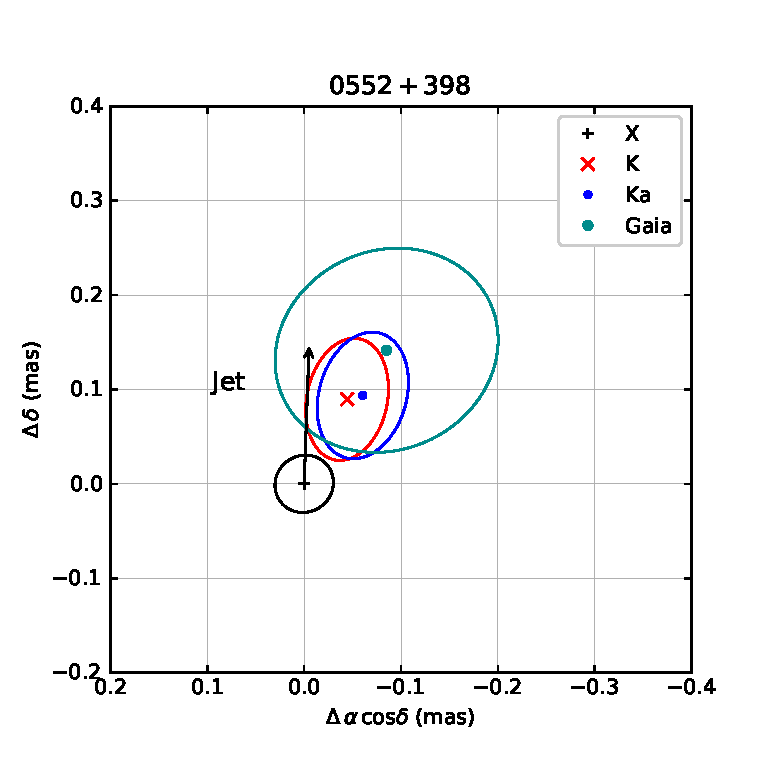
\includegraphics[width=0.45\columnwidth]{figs/0552+398}
        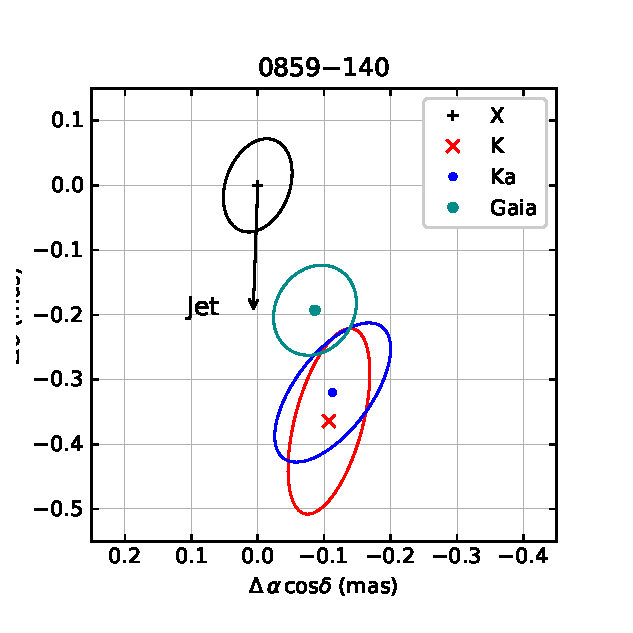
\includegraphics[width=0.45\columnwidth]{figs/0859-140}
        \includegraphics[width=0.45\columnwidth]{figs/1157-215}
        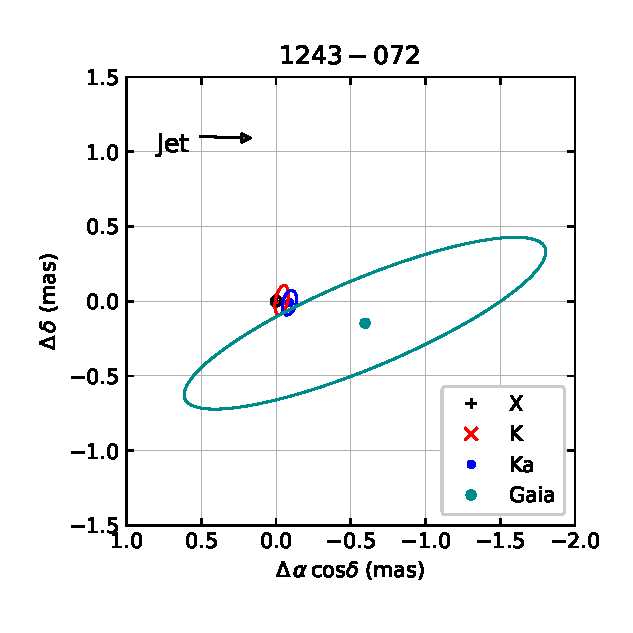
\includegraphics[width=0.45\columnwidth]{figs/1243-072}
        \includegraphics[width=0.45\columnwidth]{figs/1655+077}
        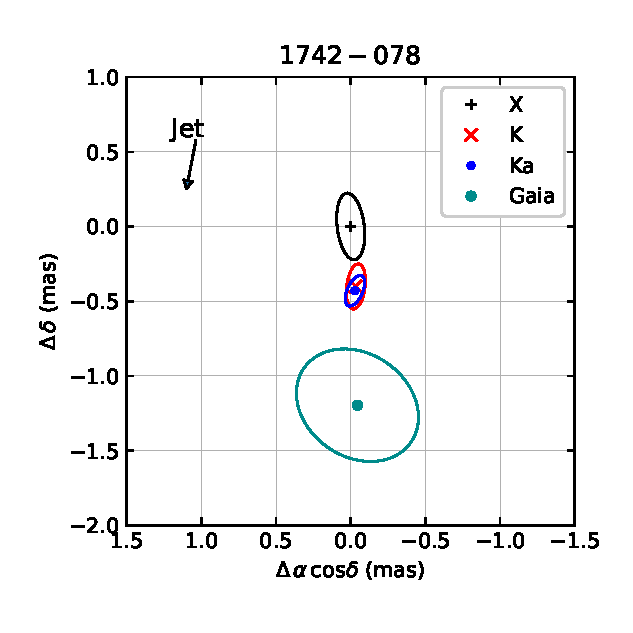
\includegraphics[width=0.45\columnwidth]{figs/1742-078}
        \includegraphics[width=0.45\columnwidth]{figs/2134+004}
        \caption[]{\label{fig:jet-down}
            Offsets of the VLBI $K$-band, $Ka$-band, and {\it Gaia} (optical) positions with respect to the VLBI $X$-band position for sources with four position aligned as in the jet downstream.
            Also shown is the jet direction of these sources taken from MOJAVE database whilst the magnitude (length) is arbitrary and thus meaningless.
        }
    \end{figure*}
%%
%__________________________________________________{fig:fig:jet-up}

    \begin{figure*}[hbtp]
        \centering
        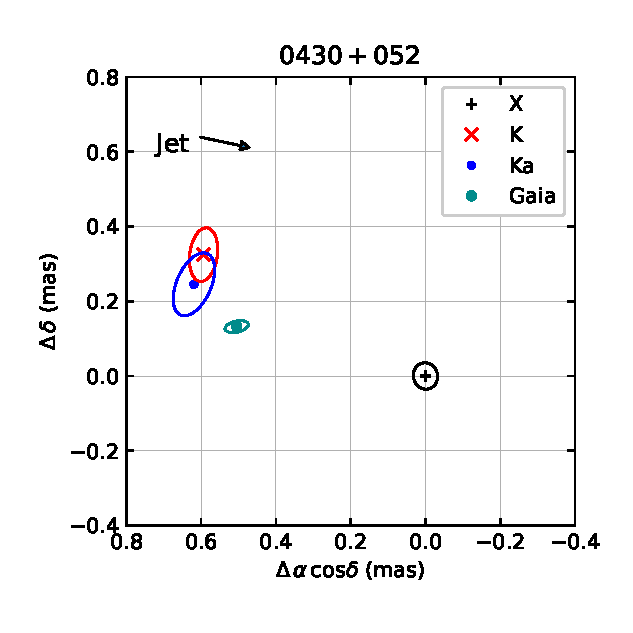
\includegraphics[width=0.45\columnwidth]{figs/0430+052}
        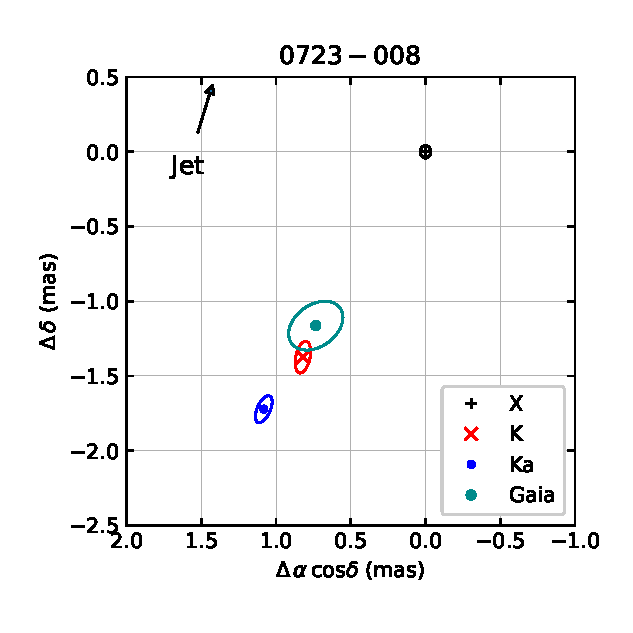
\includegraphics[width=0.45\columnwidth]{figs/0723-008}
        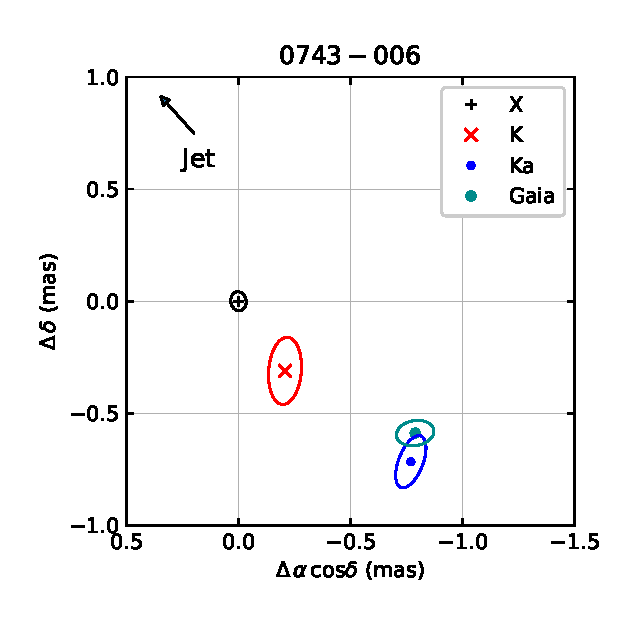
\includegraphics[width=0.45\columnwidth]{figs/0743-006}
        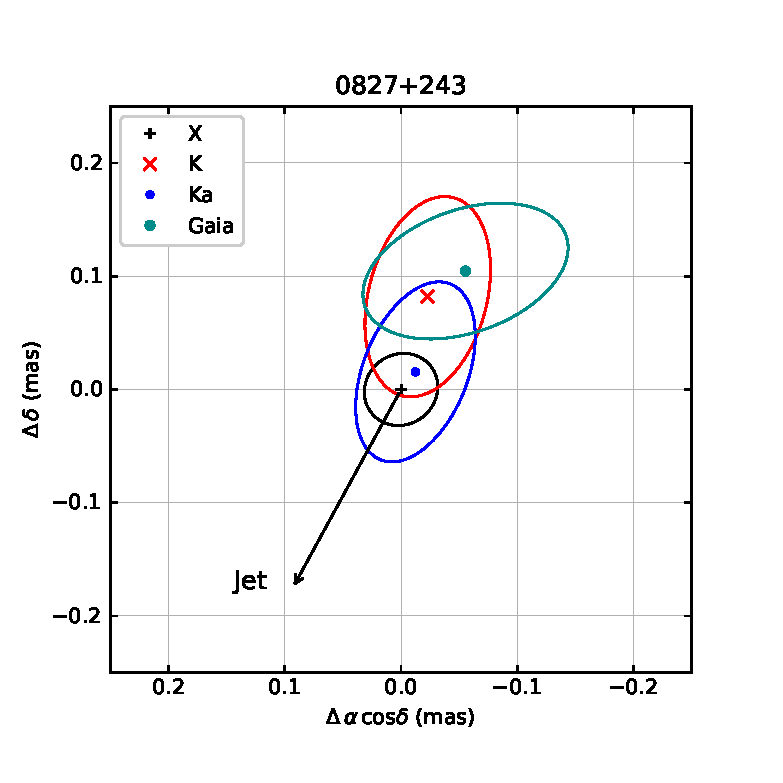
\includegraphics[width=0.45\columnwidth]{figs/0827+243}
        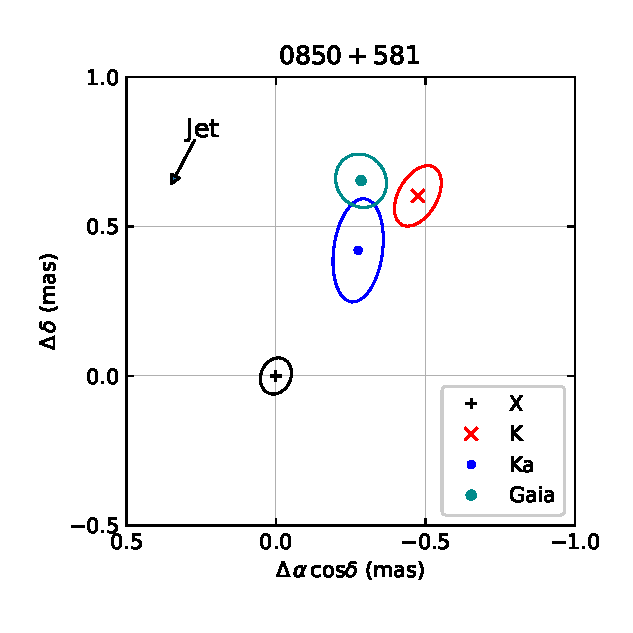
\includegraphics[width=0.45\columnwidth]{figs/0850+581}
        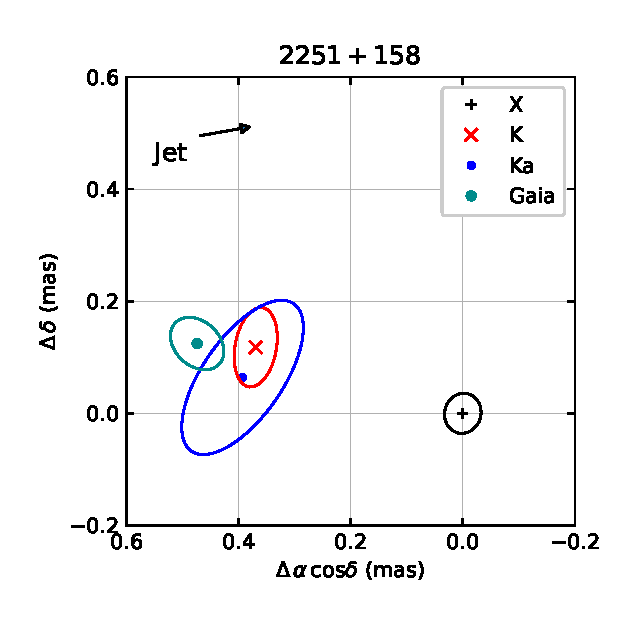
\includegraphics[width=0.45\columnwidth]{figs/2251+158}
        \caption[]{\label{fig:jet-up}
            Offsets of the VLBI $K$-band, $Ka$-band, and {\it Gaia} positions with respect to the VLBI $X$-band position for sources with four position aligned as in the jet upstream.
            Also shown is the jet direction of these sources taken from MOJAVE database whilst the magnitude (length) is arbitrary and thus meaningless.
        }
    \end{figure*}

%%
%__________________________________________________{fig:fig:jet-up}

    \begin{figure*}[hbtp]
        \centering
        \includegraphics[width=0.35\columnwidth]{figs/0003+380}
        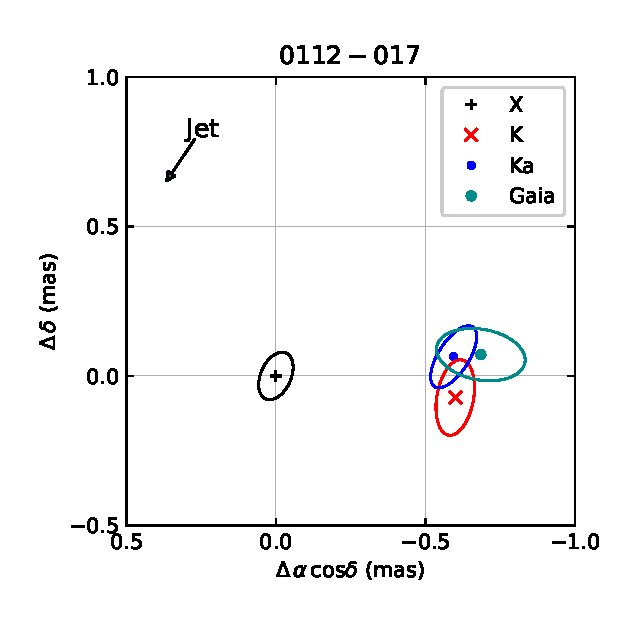
\includegraphics[width=0.35\columnwidth]{figs/0112-017}
        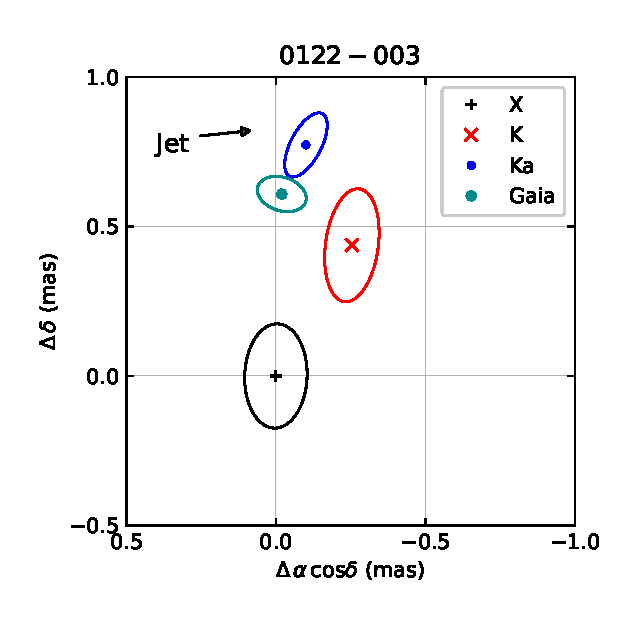
\includegraphics[width=0.35\columnwidth]{figs/0122-003}
        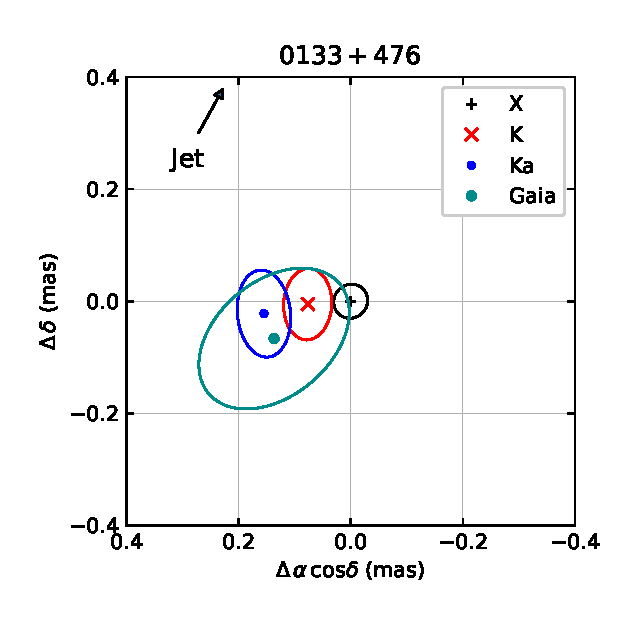
\includegraphics[width=0.35\columnwidth]{figs/0133+476}
        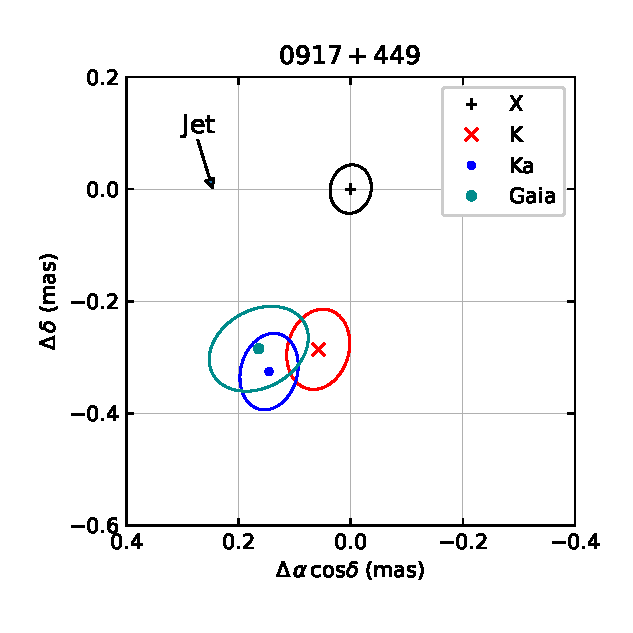
\includegraphics[width=0.35\columnwidth]{figs/0917+449}
        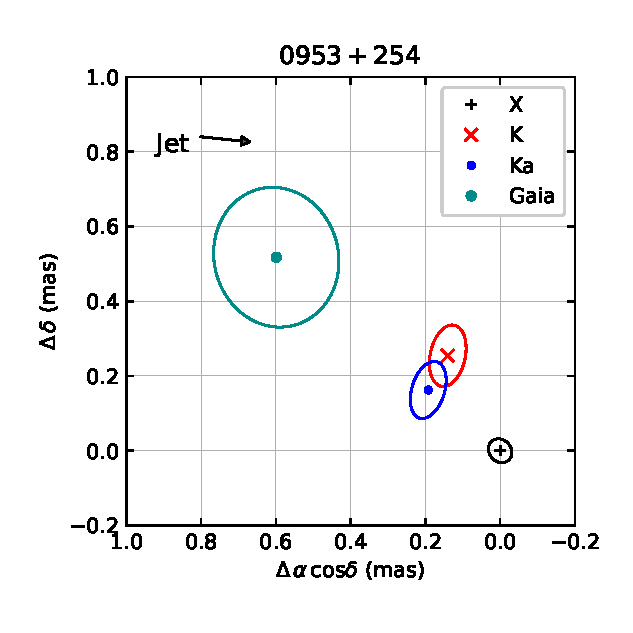
\includegraphics[width=0.35\columnwidth]{figs/0953+254}
        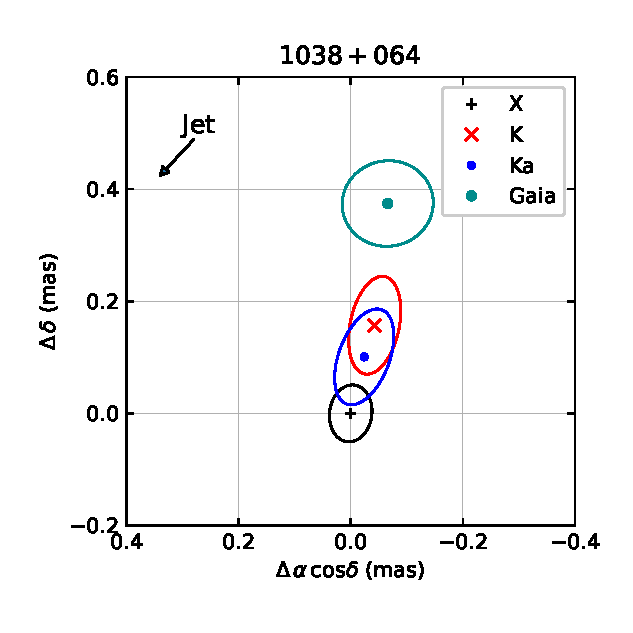
\includegraphics[width=0.35\columnwidth]{figs/1038+064}
        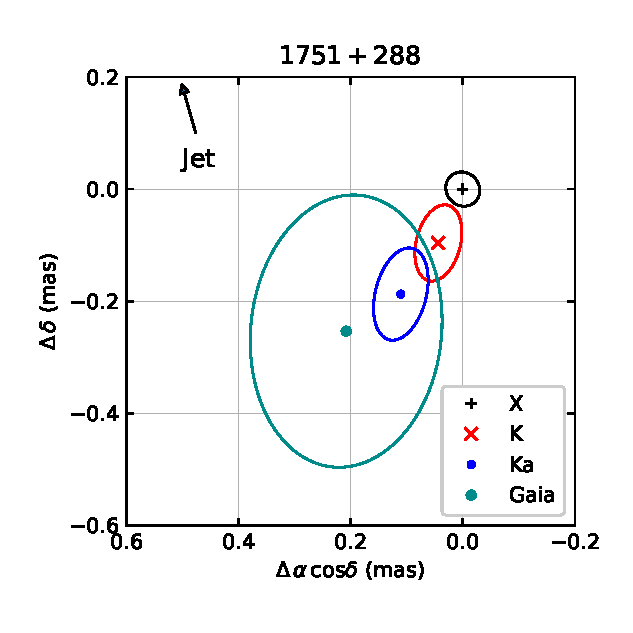
\includegraphics[width=0.35\columnwidth]{figs/1751+288}
        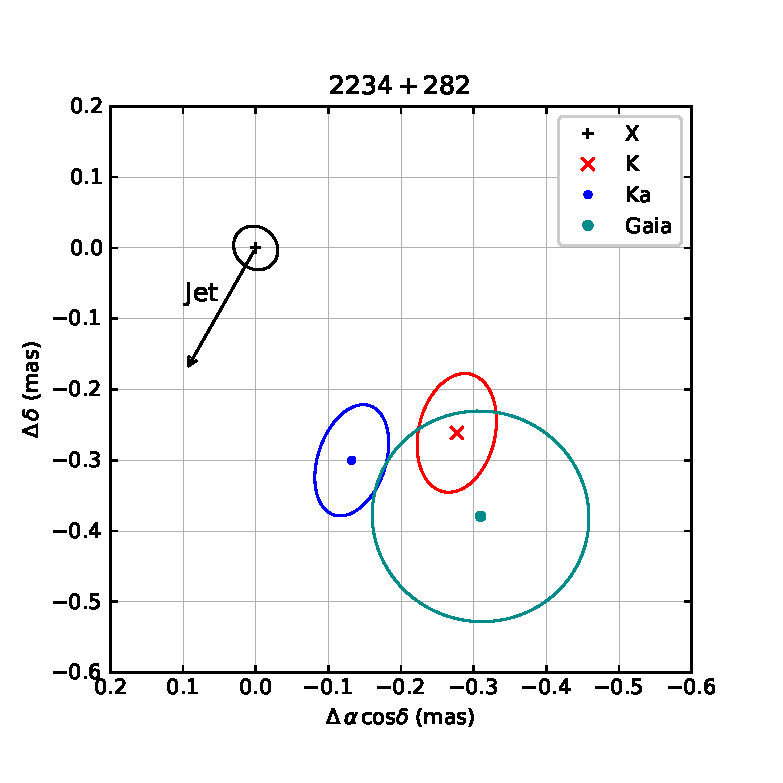
\includegraphics[width=0.35\columnwidth]{figs/2234+282}
        \caption[]{\label{fig:other}
            Offsets of VLBI $K$-band, $Ka$-band, and {\it Gaia} positions with respect to the VLBI $X$-band position for sources with four position aligned but not parallel to the jet direction.
            Also shown is the jet direction of these sources taken from MOJAVE database whilst the magnitude (length) is arbitrary and thus meaningless.
        }
    \end{figure*}

    The position offset vectors of $X$-to-$K$, $X$-to-$Ka$, and $X$-to-\textit{Gaia} are plotted for six sources with those vectors showing similar directions to the jet (Fig~\ref{fig:jet-down}), seven sources for the opposite directions (Fig~\ref{fig:jet-up}), and nine other cases (Fig~\ref{fig:other}), respectively.


\end{appendix}




\end{document}
